\documentclass[11pt,a4paper]{article}
\usepackage[margin=22mm]{geometry}
\usepackage[T1]{fontenc}
\usepackage{lmodern}
\usepackage{microtype}
\usepackage{graphicx}
\usepackage{booktabs}
\usepackage{tabularx}
\usepackage{longtable}
\usepackage{array}
\usepackage{multirow}
\usepackage{siunitx}
\usepackage{xcolor}
\usepackage{hyperref}
\usepackage{url}
\usepackage{enumitem}
\usepackage{caption}
\usepackage{subcaption}
\usepackage{float}
\usepackage{fancyhdr}
\usepackage{amsmath}
\usepackage{amssymb}
\usepackage{pifont}

\definecolor{navy}{HTML}{183B56}
\definecolor{teal}{HTML}{168C8C}
\definecolor{orange}{HTML}{D17A22}
\definecolor{lightblue}{HTML}{EDF4F7}
\definecolor{lightgray}{HTML}{F3F4F5}
\definecolor{darkgray}{HTML}{4C5661}
\hypersetup{colorlinks=true,linkcolor=navy,urlcolor=teal,citecolor=navy,pdfauthor={Felix Doublet},pdftitle={SAFE on RoboCasa: Complete Experimental Report}}
\captionsetup{font=small,labelfont=bf}
\setlist{nosep,leftmargin=1.4em}
\setlength{\parskip}{0.45em}
\setlength{\parindent}{0pt}
\setlength{\headheight}{14pt}
\renewcommand{\arraystretch}{1.15}
\graphicspath{{figures/}}
\pagestyle{fancy}
\fancyhf{}
\lhead{SAFE on RoboCasa}
\rhead{Complete experimental report}
\cfoot{\thepage}
\newcommand{\good}{\textcolor{teal}{\ding{51}}}
\newcommand{\bad}{\textcolor{orange}{\ding{55}}}
\newcommand{\code}[1]{\texttt{#1}}
\newcommand{\metric}[1]{\textbf{#1}}

\begin{document}

\begin{titlepage}
\centering
\vspace*{20mm}
{\color{navy}\rule{\textwidth}{1.4pt}}\\[12mm]
{\Huge\bfseries SAFE on RoboCasa\\[4mm]}
{\LARGE Complete Experimental Report}\\[12mm]
{\large Policy-internal failure prediction with $\pi_0$, RLDX-1, Xiaomi-Robotics-1, and semantic Subtask-SAFE}\\[16mm]
{\color{navy}\rule{\textwidth}{1.4pt}}\\[18mm]
\begin{tabular}{rl}
Period: & 13 July--15 August 2026\\
Report date: & 15 August 2026\\
Primary benchmark: & RoboCasa atomic and composite tasks\\
Primary detector families: & independent MLP and temporal LSTM\\
Evidence base: & checksum-verified archive plus frozen-holdout follow-ups\\
\end{tabular}
\vfill
\begin{minipage}{0.86\textwidth}
\small
This report records the complete experimental chain: feature instrumentation, collection and export validation, $\pi_0$ pilots, RLDX scaling, natural-prevalence and loss-weighting controls, atomic/composite ablation, semantic Subtask-SAFE, causal within-horizon objectives, targeted collection, the frozen parent-disjoint evaluation, and the Xiaomi-Robotics-1 original-SAFE study over 39 tasks. Negative results are retained because they determine the next research direction.
\end{minipage}
\vfill
{\small Felix Doublet --- Shinoda Laboratory}
\end{titlepage}

\tableofcontents
\clearpage

\section{Technical summary}

\subsection{Question}
Can SAFE-style detectors predict that a RoboCasa policy will fail early enough to support intervention, using internal action-policy features rather than only simulator state or elapsed time?

\subsection{Answer}
The integration and experimental protocol are valid, and RLDX-1 action features contain useful retrospective failure information. The strongest rollout-level RLDX MLP achieved task-normalized ROC-AUC \metric{0.713 $\pm$ 0.017} on ten tasks with 25 successes and 25 failures per task. Atomic tasks were easier than composites. At conformal $\alpha=0.20$, their balanced accuracies were \metric{0.667 $\pm$ 0.030} and \metric{0.590 $\pm$ 0.021}, respectively. Separate atomic-only and composite-only models did not improve matched performance, so mixed-task training was not the main problem.

Semantic Subtask-SAFE fixed the label mismatch for composites and achieved raw held-out segment ROC-AUC \metric{0.734 $\pm$ 0.002}. However, this result did not survive the controls required for an online claim. A causal V2 pilot, a within-horizon target, temporal feature summaries, and 320 additional targeted parents were subsequently tested. The final experiment trained with 280 parents and preserved a frozen 20-parent calibration plus 80-parent evaluation allocation. At causal prefix 32, raw features achieved ROC-AUC \metric{0.512 $\pm$ 0.003}; temporal features achieved \metric{0.566 $\pm$ 0.004}. The parent-bootstrap intervals included chance, and neither detector passed the continuation gates.

The Xiaomi-Robotics-1 extension collected 1,950 new rollouts across 39 official mid-success tasks and pooled them with 692 earlier rollouts. A deterministic 1,950-rollout training export retained 38 trainable tasks after excluding one task with only one failure. The selected MLP and LSTM completed all 810 inner-CV fits and six final refits. Training-only task normalization raised MLP outer-test ROC-AUC from \metric{0.532 $\pm$ 0.016} to \metric{0.692 $\pm$ 0.013}. In causal replay, MLP SAFE showed early within-task signal, but its 13.2\% FPR was not matched to time-only's 5.3\% FPR. The next confirmatory experiment is therefore a frozen, prospective 5\%-FPR shadow evaluation on disjoint calibration and test collections.

\begin{center}
\fcolorbox{navy}{lightblue}{\begin{minipage}{0.91\textwidth}
\textbf{Decision.} RLDX Subtask-SAFE is useful as a retrospective diagnostic but is not yet a deployable early-warning signal. Xiaomi original SAFE is more promising: its normalized MLP contains early causal ranking signal, yet no matched-FPR prospective claim exists. Freeze the Xiaomi checkpoints, normalization, time baseline, stage windows, and 5\%-FPR thresholds on a new calibration collection, then run a disjoint shadow test before any recovery intervention.
\end{minipage}}
\end{center}

\subsection{Key findings}
\begin{enumerate}
\item \good\ The $\pi_0$ and RLDX feature-capture paths are official-loader compatible and store one feature per genuine policy inference.
\item \good\ Leakage-free inner cross-validation, fixed held-out evaluation, train-only normalization, and parent-grouped splitting are operational.
\item \good\ RLDX independent MLP features rank failures within tasks; additional data improved stability.
\item \good\ The normal RLDX alpha sweep reproduces the SAFE paper's balanced-accuracy--detection-time evaluation geometry, with misses counted at normalized time 1.
\item \bad\ The LSTM was consistently weaker than the independent MLP at these sample sizes.
\item \bad\ Natural prevalence and official inverse-frequency weighting changed results only marginally.
\item \bad\ Separate atomic/composite models did not beat the mixed model.
\item \bad\ Raw Subtask-SAFE ROC was inflated by task/subtask score offsets, unequal priors, and late segment information.
\item \bad\ SAFE did not beat task-conditioned elapsed time in causal-prefix or conformal operation.
\item \bad\ Strong inner-CV results for within-horizon and temporal representations did not transfer to the frozen four-stage evaluation.
\item \good\ Xiaomi original SAFE completed a 39-task collection and a leakage-controlled 810-fit search; task normalization materially improved MLP ranking.
\item \good\ Xiaomi MLP SAFE showed task-macro causal ROC-AUC 0.671 at 10\% and 0.626 at 25\% of task horizon, above the within-task time-only value of 0.5.
\item \bad\ The opened Xiaomi replay did not compare SAFE and time at the same false-positive budget; its promising early alarms therefore remain post-hoc.
\end{enumerate}

\section{Scope, labels, and experimental rules}

\subsection{Two prediction units}
\textbf{Rollout SAFE} uses the official binary label: success if the RoboCasa terminal task predicate becomes true, otherwise failure at the horizon. \textbf{Subtask-SAFE} predicts whether the current ordered natural-language subtask eventually fails before completion.

One feature record is stored per genuine policy inference. Cached actions from a predicted chunk do not create duplicate feature records. This prevents action-reuse frequency from becoming an accidental sampling weight.

\subsection{Models and selectors}
The official SAFE detector families were retained:
\begin{itemize}
\item \code{indep}: an independent MLP detector;
\item \code{lstm}: a temporal LSTM detector.
\end{itemize}
Hyperparameters include horizon selector, diffusion selector, learning rate, and regularization. Unless explicitly noted, the search used three inner folds and model seeds 0, 1, and 2.

\subsection{Evaluation contract}
\begin{itemize}
\item Outer test identities are fixed and never used for hyperparameter selection.
\item Normalization statistics are fitted from training data only.
\item Subtask segments are split by parent rollout before extraction.
\item Raw pooled ROC/AP, task-normalized pooled ROC/AP, and macro task ROC/AP are kept distinct.
\item Duration or elapsed-time baselines are mandatory.
\item A conformal lead time is reported only together with the TPR that determines how often that lead is obtained.
\end{itemize}

\section{Feature instrumentation and system validation}

\subsection{\texorpdfstring{$\pi_0$}{pi0} RoboCasa}
The $\pi_0$ integration captures the official SAFE \code{pre\_velocity} feature: action-expert suffix hidden states immediately before \code{action\_out\_proj}. The expected tensor is $10\times50\times1024$ (flow steps, action tokens, channels). Pinned instrumentation:
\begin{quote}\small
OpenPI commit: \path{5a6beda9ff99da30b4e1b59320f6a32971d7c397}\\
Patch: \path{patches/openpi_safe_features_5a6beda.patch}
\end{quote}

The first smoke failed correctly because the policy server did not return \code{safe\_features}. After applying the patch to the pinned server and enabling feature return, a sink smoke produced two successes and one failure and passed the official loader.

\subsection{RLDX-1}
RLDX has no literal \code{action\_expert} module. The selected analogous action stream is \code{ao[:, -action\_horizon:]} immediately before the embodiment-specific decoder. Its layer identifier is \code{action\_model\_msat\_action\_suffix\_pre\_action\_decoder}; observed shape is $4\times16\times1024$.
\begin{quote}\small
Model: \path{RLWRLD/RLDX-1-FT-RC365}\\
Repository commit: \path{ef05cd4ae634ff97d672d42275febbc0b92cc192}
\end{quote}

Two ZeroMQ servers were validated on ports 20100 and 20101. A nested language-batch shape bug was corrected: flat request fields use \code{[instruction]}, while nested direct-policy language uses \code{[[instruction]]}.

\subsection{Xiaomi-Robotics-1}
The Xiaomi integration preserves the released RoboCasa365 policy behavior and
adds an opt-in SAFE response. At each genuine inference it records the final
DiT-layer action-token state immediately before the action output projection.
The feature identifier is:
\begin{quote}\small
\path{dit_action_tokens_pre_action_output_layer}
\end{quote}
Its observed tail shape is $5\times30\times1024$ (flow steps, action tokens,
channels). One inference,
not each cached action, creates one SAFE feature record. Pinned artifacts are:
\begin{quote}\small
Xiaomi repository commit:
\path{4da1db0a4deefa6de7ebb4ef0b8754017290f5f7}\\
Checkpoint revision:
\path{0d1aa76d0d82debc9b611e4d1e231096434d5be4}\\
Transformers: 4.57.1; action replanning interval: 16.
\end{quote}
The official evaluation preprocessing was retained: \code{pretrain} split,
observation history 4, interval 2, and crop ratio 0.95. The policy server and
simulator client use separate processes and ports 10096 and 10097 for
two-GPU collection.

\subsection{ABot-M0.5}
An ABot-M0.5 adapter was implemented with the same explicit request/response contract and inference-aligned capture rule. No ABot detector-training result is included here; it remains an engineering-only extension and must not be interpreted as evidence of model performance.

\section{Dataset chronology and audits}

\begin{longtable}{p{0.22\textwidth}p{0.18\textwidth}p{0.49\textwidth}}
\toprule
Dataset/phase & Outcome & Evidence and interpretation\\
\midrule
\endfirsthead
\toprule
Dataset/phase & Outcome & Evidence and interpretation\\
\midrule
\endhead
$\pi_0$ sink smoke & 3 rollouts & 2 successes, 1 failure; feature server and official loader validated.\\
$\pi_0$ first five-task attempt & invalid protocol & Wrong split/policy setup yielded only failures; discarded as scientific evidence.\\
$\pi_0$ five-task official & 118 retained & 60 successes, 58 failures; exact 10/10-per-task export derived from the healthy pool.\\
$\pi_0$ 17-atomic expansion & incomplete & Asset and server failures preserved; not used in training claims.\\
RLDX 10-task pilot & 200 retained & 100 successes, 100 failures; 10/10 per task; five atomic and five composite tasks.\\
RLDX expanded & 500 retained & 250 successes, 250 failures; 25/25 per task; official export 15 GiB.\\
Natural-rate pool & 689 outcomes & Genuine observed outcomes used to construct five immutable subsets with 23 training examples per task.\\
Subtask-SAFE parents & 150 rollouts & 65 successful, 85 failed parents; semantic decomposition into 18 task/subtask identities.\\
Subtask-SAFE segments & 426 usable & 341 successful, 85 failed; 27,420 policy records; official-loader compatible.\\
V2 targeted pilot & 80 parents & Twenty new rollouts for each of four composite tasks; 36 successes, 44 failures; 257 semantic segments.\\
V2 long collection & 320 parents & 290-rollout long batch plus 30 additional WashLettuce rollouts; all valid, with 202 failures and 118 successes.\\
V2 frozen allocation & 100 parents & Twenty calibration parents and 80 evaluation parents, exactly 10 successful and 10 failed target-stage parents per stage; identities frozen before final refits.\\
V2 augmented training & 280 parents & Original training parents plus 180 previously unassigned new-seed parents; frozen calibration and evaluation identities unchanged.\\
Xiaomi ten-task pool & 692 rollouts & 419 successes and 273 failures; deterministic 25/25-per-task export contained 500 rollouts.\\
Xiaomi official mid-success collection & 1,950 rollouts & Exactly 50 rollouts for each of 39 tasks; 1,106 successes and 844 failures; all artifacts and official loading validated.\\
Xiaomi pooled training export & 1,950 rollouts & Selected from a 2,642-rollout source pool; 1,105 successes and 845 failures; 38 tasks used for training after one sparse-failure exclusion.\\
\bottomrule
\end{longtable}

The report bundle itself contains 20,857 archive entries and passed SHA-256 verification. Incomplete and quarantined artifacts are retained as provenance rather than silently deleted.

\section{\texorpdfstring{$\pi_0$}{pi0} experiments}

\subsection{Training and evaluator smokes}
Independent and LSTM two-epoch evaluator smokes first established that the official SAFE loader, detector checkpoints, and offline evaluator agreed. A two-configuration 1,000-epoch grid pilot then confirmed that the apparently short wall time was expected: with roughly 100 rollouts and batch size 512, one epoch is only a small full-batch update. These runs were engineering gates, not performance claims.

An initial six-run all-five-seen fit, before leakage-free hyperparameter selection, produced MLP ROC $0.506\pm0.009$ and PRC $0.541\pm0.019$, versus LSTM ROC $0.702\pm0.031$ and PRC $0.675\pm0.025$. It motivated the full inner-CV experiment but was superseded by the fixed-split result below.

\subsection{Official 810-fit grid}
All 810 runs completed (270 configurations, three seeds). The selected MLP achieved seen validation ROC \metric{0.799 $\pm$ 0.081}, while its unseen value was \metric{0.453 $\pm$ 0.037}. The LSTM achieved seen \metric{0.792 $\pm$ 0.069} and unseen \metric{0.581 $\pm$ 0.080}. These are validation results from a small 100-rollout dataset, not a final held-out estimate.

\begin{figure}[H]
\centering
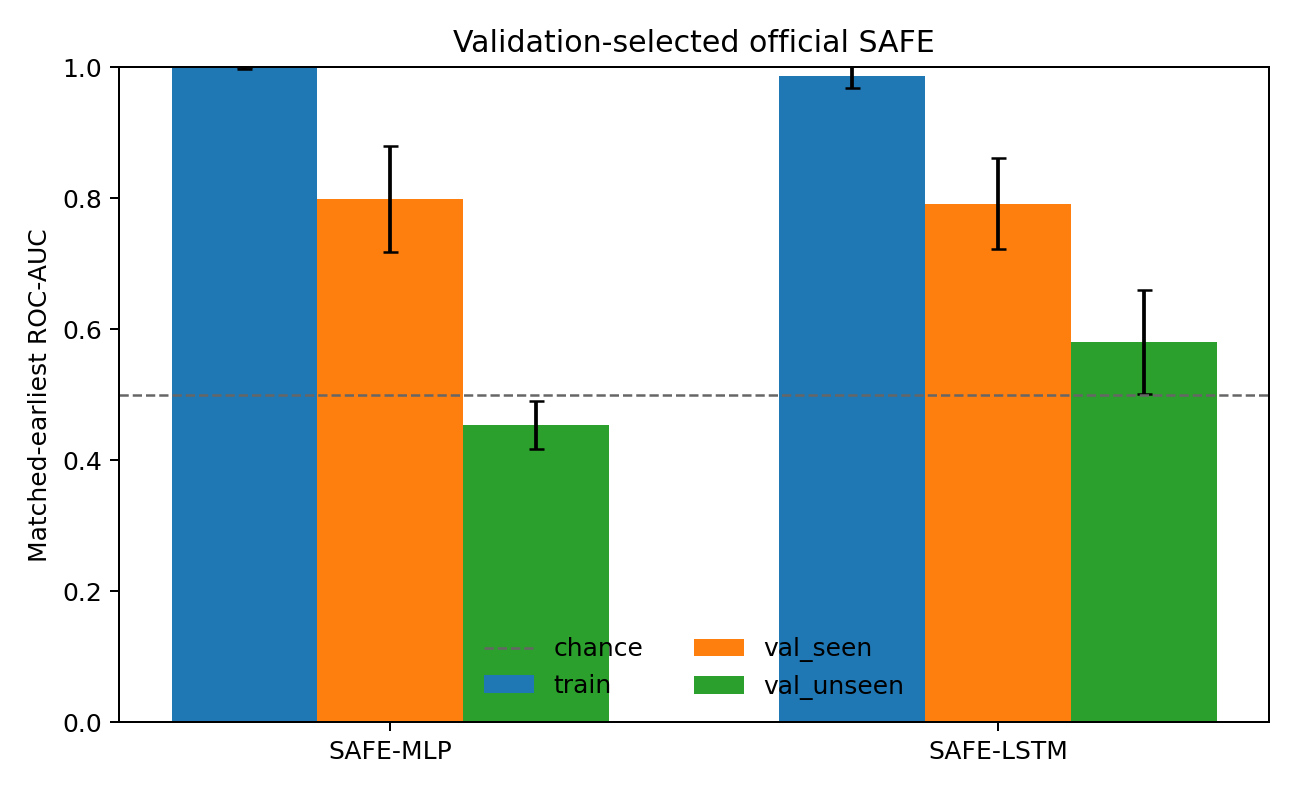
\includegraphics[width=0.88\textwidth]{pi0_official_selected_auc.png}
\caption{$\pi_0$ official-grid selection. Seen-task validation is substantially stronger than unseen-task validation, but uncertainty across seeds is high.}
\label{fig:pi0grid}
\end{figure}

Conformal operation remained weak. At $\alpha=0.15$, the MLP had TPR 0.300 and FPR 0.383; the LSTM had TPR 0.183 and FPR 0.150. Neither produced a convincing intervention point.

\subsection{Leakage-free five-task experiment}
The outer split used 70 training rollouts and 30 held-out rollouts, balanced within each of five atomic tasks. Inner-CV selected MLP ROC \metric{0.719 $\pm$ 0.021} and LSTM ROC \metric{0.817 $\pm$ 0.034}. Final held-out results were:

\begin{table}[H]
\centering
\caption{$\pi_0$ leakage-free final results (three model seeds).}
\begin{tabular}{lcc}
\toprule
Model & Test ROC-AUC & Test PRC-AUC\\
\midrule
Independent MLP & 0.600 $\pm$ 0.004 & 0.605 $\pm$ 0.002\\
LSTM & 0.599 $\pm$ 0.039 & 0.637 $\pm$ 0.031\\
\bottomrule
\end{tabular}
\end{table}

\begin{figure}[H]
\centering
\begin{subfigure}{0.49\textwidth}
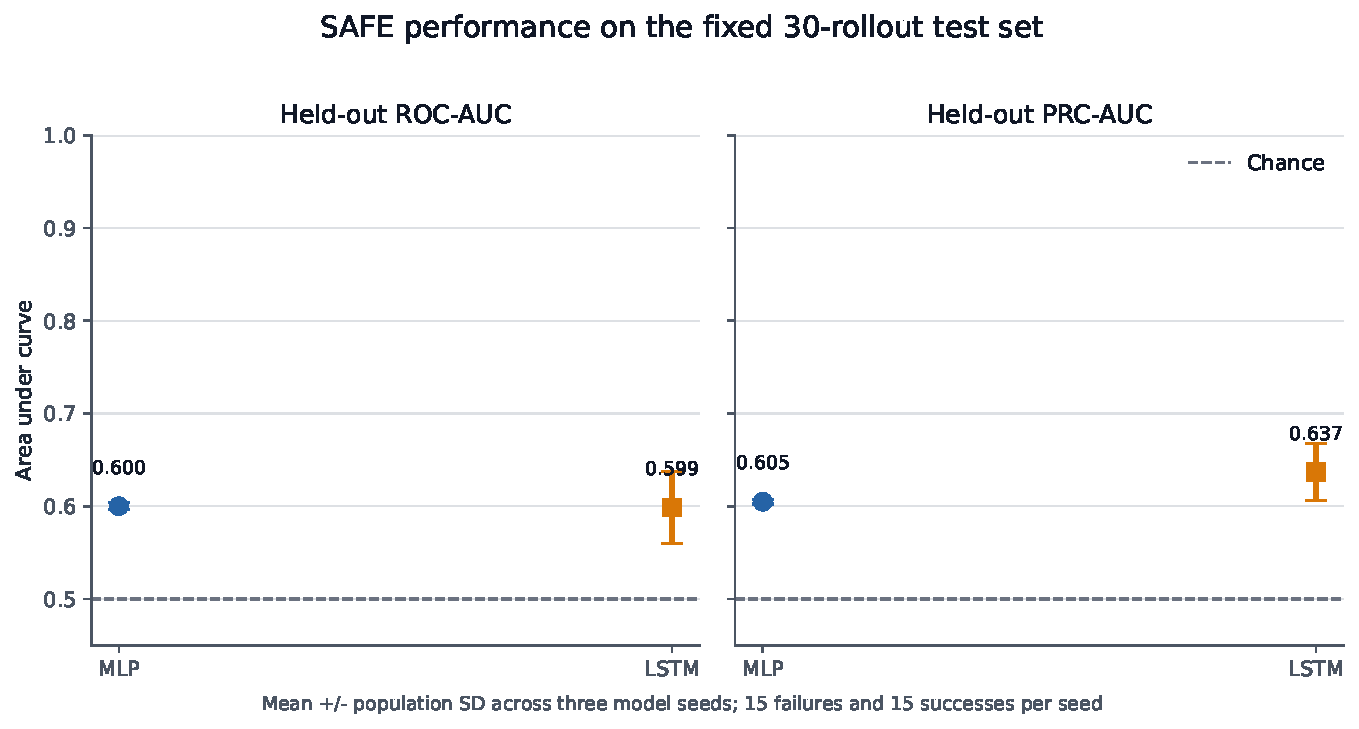
\includegraphics[width=\textwidth]{pi0_leakage_free_test_auc.pdf}
\caption{Held-out ROC and PRC.}
\end{subfigure}\hfill
\begin{subfigure}{0.49\textwidth}
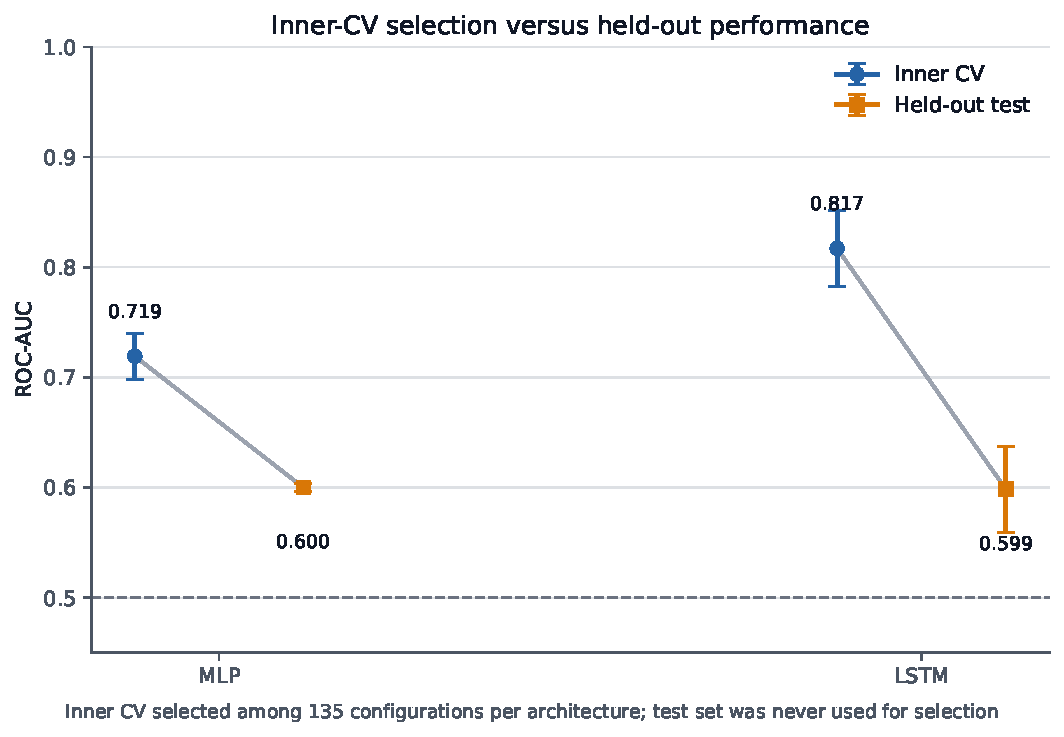
\includegraphics[width=\textwidth]{pi0_cv_to_test_gap.pdf}
\caption{Inner-CV to test gap.}
\end{subfigure}
\caption{Leakage-free $\pi_0$ evaluation. Stronger inner validation did not transfer to the small held-out set.}
\end{figure}

\section{RLDX rollout-level experiments}

\subsection{Scaling from 10/10 to 25/25 per task}
Ten tasks were used: five atomic and five composite. Increasing from 20 to 50 rollouts per task improved the independent MLP's within-task ranking and reduced variance.

\begin{table}[H]
\centering
\caption{RLDX held-out discrimination as data increased.}
\begin{tabular}{llcc}
\toprule
Dataset & Model & Raw pooled ROC & Train-only task-z ROC\\
\midrule
10/10 per task & MLP & 0.543 $\pm$ 0.007 & 0.674 $\pm$ 0.023\\
10/10 per task & LSTM & 0.520 $\pm$ 0.025 & 0.537 $\pm$ 0.026\\
25/25 per task & MLP & 0.575 $\pm$ 0.004 & \textbf{0.713 $\pm$ 0.017}\\
25/25 per task & LSTM & 0.554 $\pm$ 0.006 & 0.547 $\pm$ 0.010\\
\bottomrule
\end{tabular}
\end{table}

\begin{figure}[H]
\centering
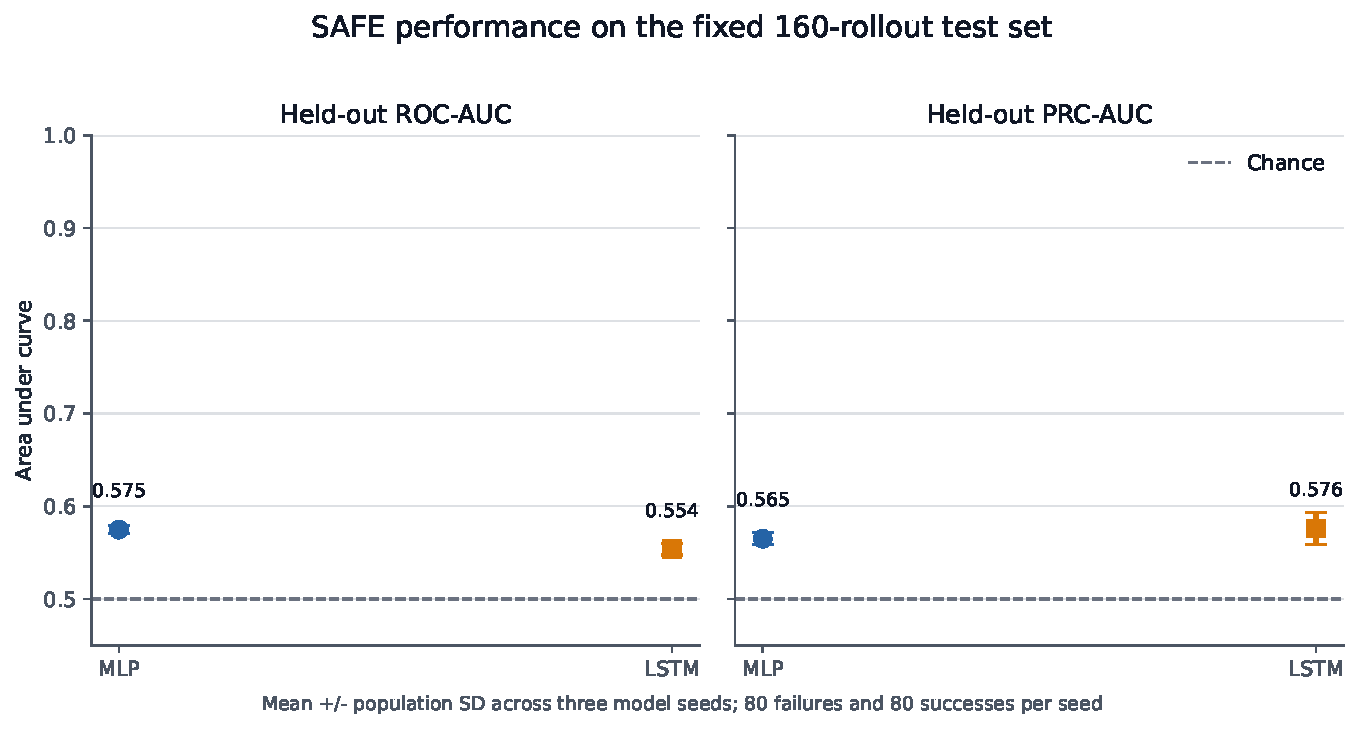
\includegraphics[width=0.78\textwidth]{rldx25_test_auc.pdf}
\caption{RLDX 25/25 final held-out metrics. The MLP is stable across seeds; the LSTM remains weaker.}
\end{figure}

The large raw-to-task-z gap means a global score is not directly comparable across tasks. Task normalization is reasonable as an analysis and calibration tool when task identity is known, but it is not evidence that the raw detector is globally calibrated.

\subsection{Rollout-level conformal calibration}
The 500-rollout dataset was divided into 340 training rollouts, 30 calibration successes, and 130 evaluation rollouts. At $\alpha=0.15$, the MLP achieved TPR 0.196, FPR 0.040, and balanced accuracy 0.578. The originally archived detection-time value 0.716 was conditional on a failure being detected. Under the paper definition, an undetected failed rollout has normalized detection time 1, giving a paper-equivalent average of approximately 0.944. Recall therefore remained too low for reliable recovery.

\subsection{Expanded alpha sweep and paper-equivalent timeliness}
The functional conformal sweep was extended from $\alpha\leq0.20$ to $\alpha\leq0.50$. Increasing $\alpha$ lowers conservativeness, usually increasing both detection coverage and false alarms. Because the official \code{tfunc} modulation itself depends on $\alpha$, the resulting functional bands are not guaranteed to be nested; small non-monotonic changes are therefore possible.

\begin{table}[H]
\centering
\caption{Task-normalized RLDX MLP operating points. Accuracy is ordinary accuracy; balanced accuracy is the primary metric because each type-specific evaluation set contains 40 failures and 25 successes per seed.}
\resizebox{\textwidth}{!}{%
\begin{tabular}{llcccc}
\toprule
Type & $\alpha$ & Accuracy & Balanced accuracy & TPR & FPR\\
\midrule
Atomic & 0.15 & $0.533\pm0.015$ & $0.608\pm0.015$ & 0.283 & 0.067\\
Atomic & 0.20 & $0.615\pm0.038$ & $0.667\pm0.030$ & 0.442 & 0.107\\
Atomic & 0.35 & $0.703\pm0.032$ & $\mathbf{0.683\pm0.015}$ & 0.767 & 0.400\\
Atomic & 0.50 & $0.708\pm0.045$ & $0.640\pm0.048$ & 0.933 & 0.653\\
\midrule
Composite & 0.15 & $0.446\pm0.013$ & $0.547\pm0.007$ & 0.108 & 0.013\\
Composite & 0.20 & $0.508\pm0.022$ & $\mathbf{0.590\pm0.021}$ & 0.233 & 0.053\\
Composite & 0.35 & $0.487\pm0.071$ & $0.551\pm0.053$ & 0.275 & 0.173\\
Composite & 0.50 & $0.554\pm0.044$ & $0.590\pm0.032$ & 0.433 & 0.253\\
\bottomrule
\end{tabular}}
\label{tab:rldx-alpha}
\end{table}

At $\alpha=0.20$, the combined ten-task detector had TPR 0.337, FPR 0.080, and balanced accuracy 0.629. Atomic $\alpha=0.35$ is the best point under the paper's two plotted objectives, but its 40\% false-positive rate is unsuitable for routine intervention. Composite $\alpha=0.50$ attains the same balanced accuracy as $\alpha=0.20$ with nearly five times the FPR. The practical shared operating point remains $\alpha=0.20$; the extended curve is a post-hoc sensitivity analysis, not a new confirmatory selection.

The SAFE paper defines $T_{\mathrm{det}}$ as the first threshold-crossing timestep divided by the failed rollout duration, assigns $T_{\mathrm{det}}=1$ to misses, and averages over ground-truth failed rollouts~\cite{gu2026safe}. Figure~\ref{fig:rldx-paper-tradeoff} reconstructs that metric from the archived confusion counts and conditional detection times. It reproduces the paper's evaluation geometry, not its complete benchmark: no human failure-onset annotations or competing baselines are available here.

\begin{figure}[H]
\centering
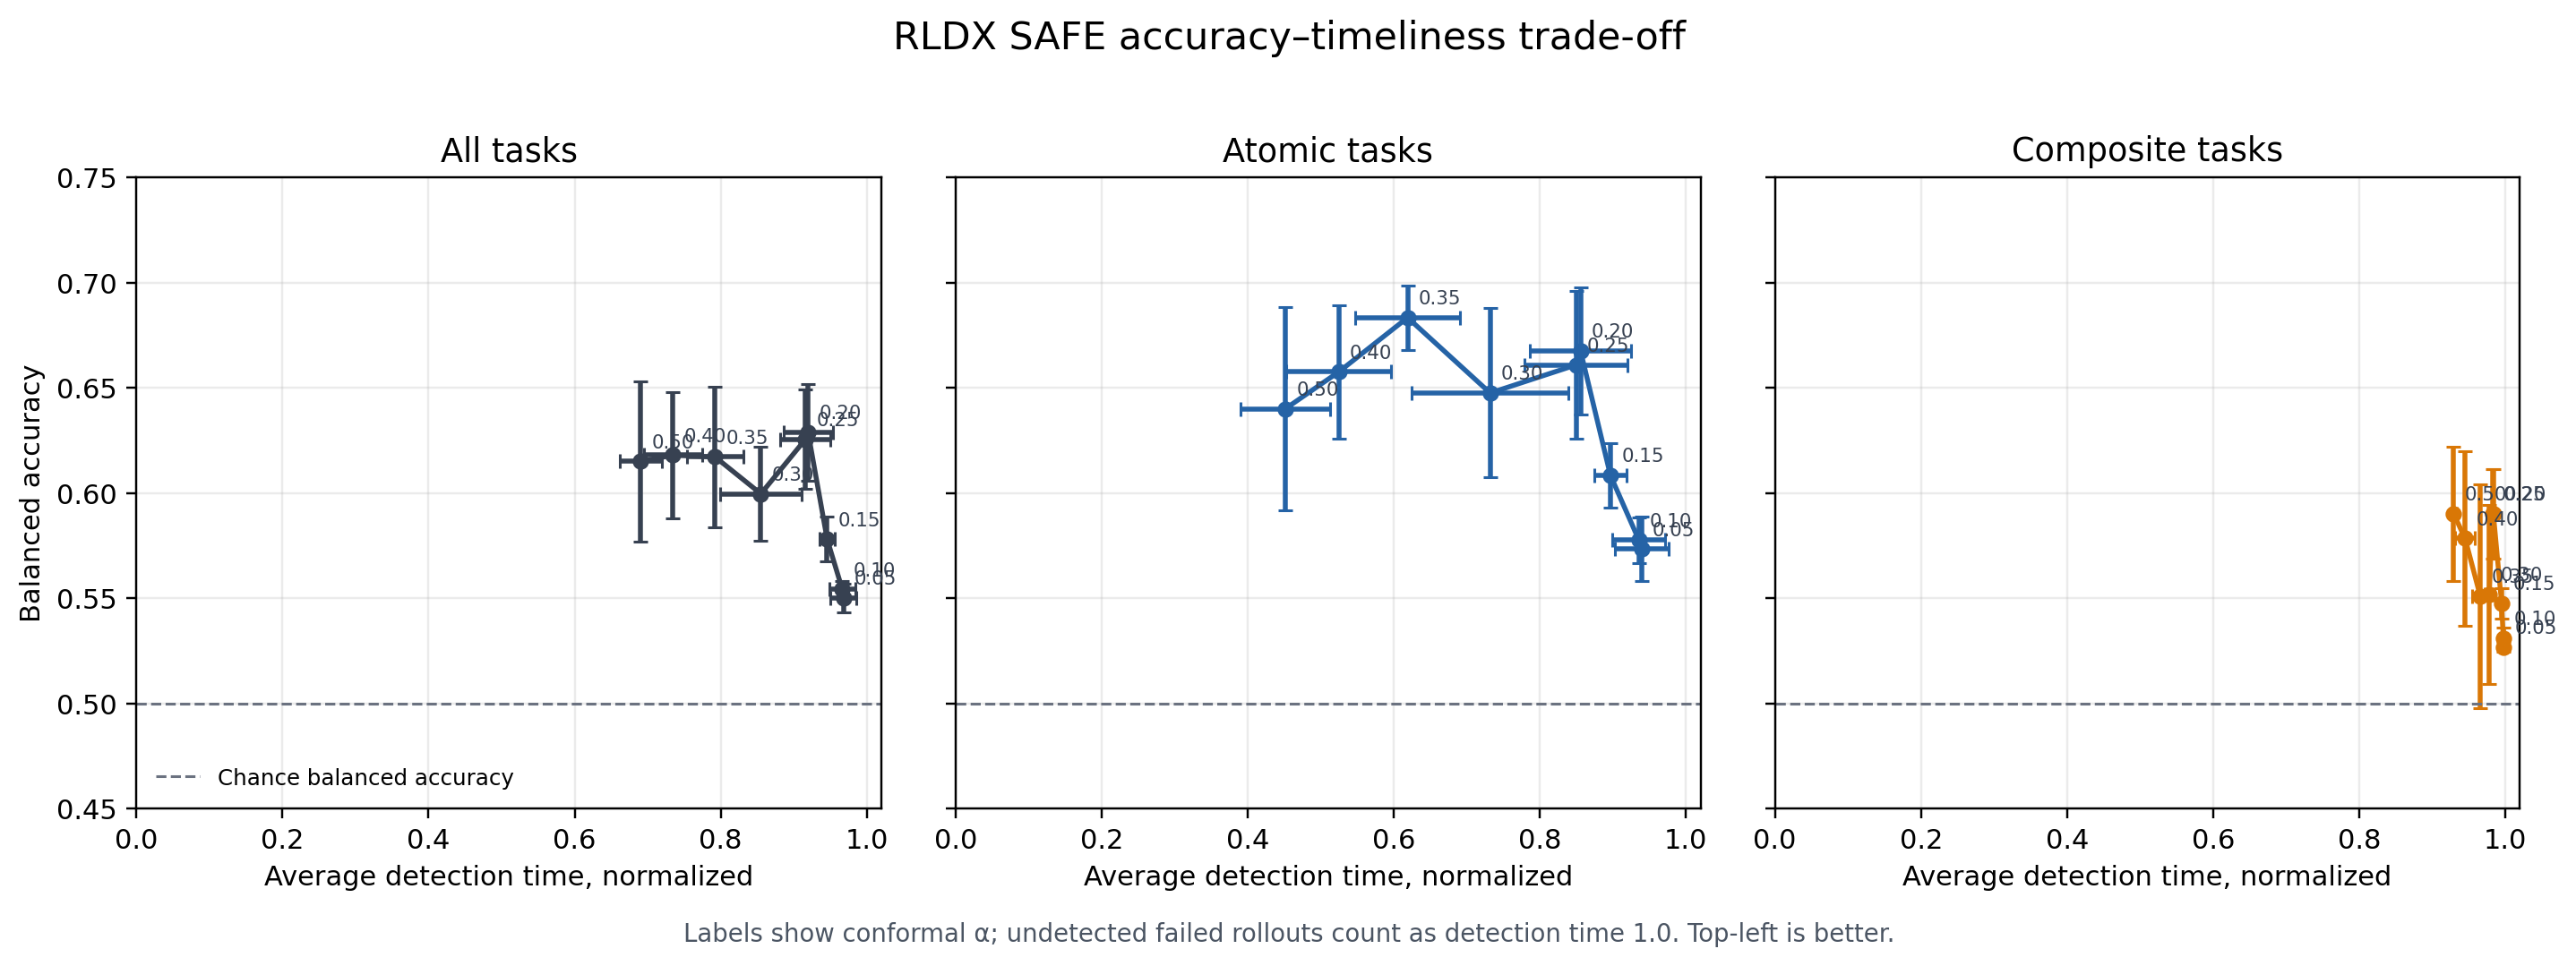
\includegraphics[width=\textwidth]{rldx_normal_safe_paper_tradeoff.png}
\caption{Paper-style balanced-accuracy--timeliness curves for task-normalized RLDX SAFE-MLP. Labels are conformal $\alpha$; misses count as normalized time 1. Atomic tasks form a useful frontier, whereas composite failures are generally detected near the horizon or missed. Error bars are population standard deviations across three model seeds on one fixed evaluation set.}
\label{fig:rldx-paper-tradeoff}
\end{figure}

\subsection{Comparison with the SAFE paper}
The original SAFE simulation study evaluated unseen tasks and reported ROC-AUC over the rollout maximum score. Its unseen-task SAFE-MLP ROC ranged from 0.733 on $\pi_0$+LIBERO to 0.848 on $\pi_0^*$+SimplerEnv; SAFE-LSTM ranged from 0.711 to 0.845~\cite{gu2026safe}. The RLDX result uses held-out samples from the same ten tasks and training-only task-z normalization, so it is a seen-task conditional result rather than a zero-shot reproduction.

\begin{table}[H]
\centering
\caption{SAFE paper unseen-task ROC-AUC and the present RLDX seen-task result. The protocols, policies, tasks, feature layers, and normalization differ; the last row is contextual, not a controlled ranking.}
\begin{tabular}{lcc}
\toprule
Policy and benchmark & SAFE-MLP & SAFE-LSTM\\
\midrule
OpenVLA + LIBERO, unseen & 0.735 & 0.725\\
$\pi_0$-FAST + LIBERO, unseen & 0.804 & 0.845\\
$\pi_0$ + LIBERO, unseen & 0.733 & 0.711\\
$\pi_0^*$ + SimplerEnv, unseen & 0.848 & 0.801\\
\midrule
RLDX-1 + RoboCasa, seen task-z & 0.713 & 0.547\\
RLDX-1 + RoboCasa, seen raw pooled & 0.575 & 0.554\\
\bottomrule
\end{tabular}
\label{tab:safe-paper-compare}
\end{table}

\begin{figure}[H]
\centering
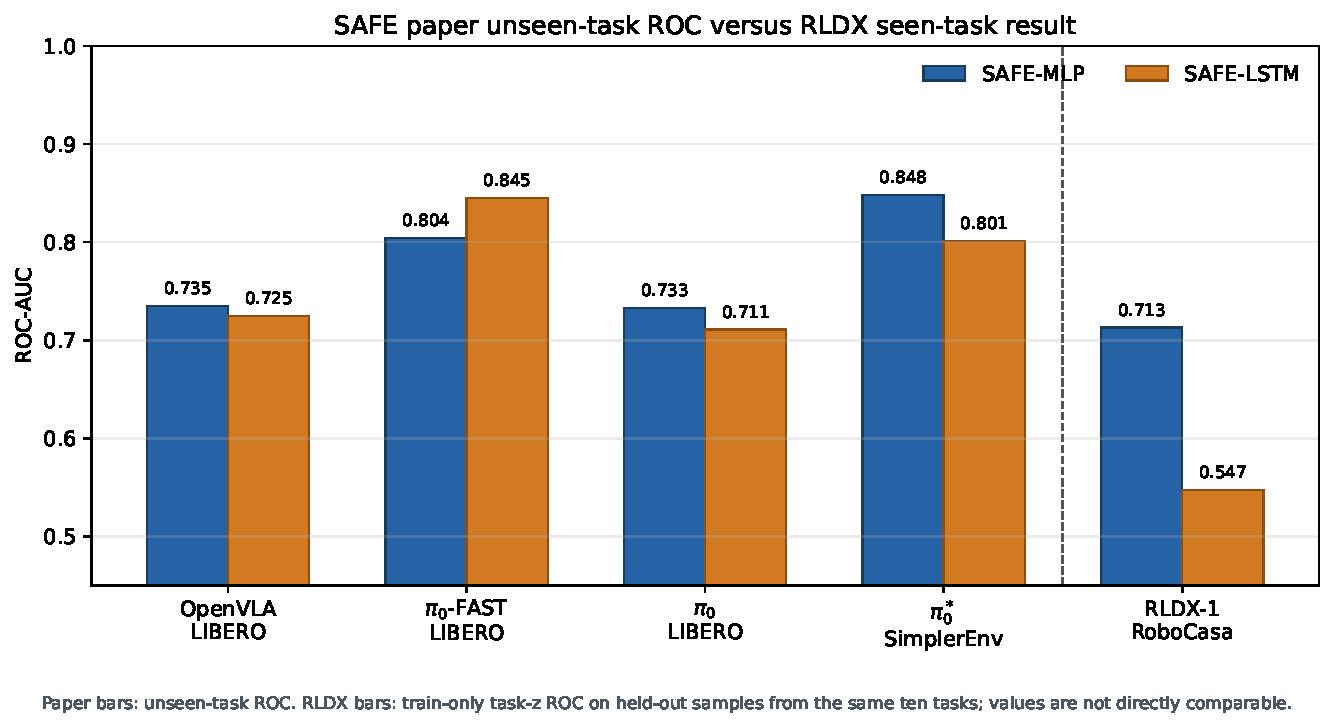
\includegraphics[width=0.94\textwidth]{safe_paper_rldx_roc_comparison.pdf}
\caption{Contextual ROC comparison. The dashed separator emphasizes that the SAFE-paper bars are unseen-task results, whereas RLDX uses held-out samples from known tasks and task-conditioned normalization.}
\label{fig:safe-paper-roc}
\end{figure}

The RLDX MLP task-z ROC 0.713 is numerically close to the paper's $\pi_0$+LIBERO unseen MLP ROC 0.733, but the similarity must not be interpreted as reproduced generalization. Raw RLDX pooling is materially weaker, the LSTM does not transfer, and the conformal composite-task curve lies near $T_{\mathrm{det}}=1$. Relative to the paper, the principal deficit is therefore not only retrospective ranking but the conversion of scores into timely, task-robust failure alarms.

\subsection{Atomic versus composite ablation}
The mixed MLP was stronger on atomic tasks (task-z ROC 0.827) than composites (0.667). Separate models did not improve matched evaluation:

\begin{table}[H]
\centering
\caption{Matched mixed-versus-type-specific MLPs at $\alpha=0.15$.}
\begin{tabular}{llccccc}
\toprule
Type & Model & Task-z ROC & Task-z PRC & TPR & FPR & Bal. acc.\\
\midrule
Atomic & Mixed & 0.827 & 0.891 & 0.275 & 0.027 & 0.624\\
Atomic & Split & 0.821 & 0.880 & 0.217 & 0.133 & 0.542\\
Composite & Mixed & 0.667 & 0.773 & 0.167 & 0.067 & 0.550\\
Composite & Split & 0.668 & 0.777 & 0.192 & 0.107 & 0.543\\
\bottomrule
\end{tabular}
\end{table}

This rejects the hypothesis that mixing short- and long-horizon tasks is the main source of confusion. It instead motivates finer temporal labels for composites.

\section{Natural prevalence and paper-style weighting}

The natural-rate study compared matched balanced weighting, natural unweighted training, and natural training with official inverse-frequency weighting. Five subset seeds and three model seeds produced 90 completed runs on one immutable 160-rollout test set.

\begin{table}[H]
\centering
\caption{Natural-prevalence study. AP denotes average precision.}
\resizebox{\textwidth}{!}{%
\begin{tabular}{llcccccc}
\toprule
Model & Regime & Raw ROC & Task-z ROC & Macro ROC & Raw AP & Task-z AP & Macro AP\\
\midrule
MLP & Matched weighted & 0.566 & 0.691 & 0.694 & 0.572 & 0.713 & 0.743\\
MLP & Natural unweighted & \textbf{0.573} & \textbf{0.700} & 0.714 & 0.568 & 0.721 & 0.748\\
MLP & Natural weighted & 0.571 & 0.699 & \textbf{0.715} & 0.563 & \textbf{0.726} & \textbf{0.751}\\
LSTM & Matched weighted & \textbf{0.546} & \textbf{0.538} & \textbf{0.556} & \textbf{0.579} & \textbf{0.556} & 0.645\\
LSTM & Natural unweighted & 0.525 & 0.522 & 0.553 & 0.564 & 0.532 & \textbf{0.647}\\
LSTM & Natural weighted & 0.532 & 0.529 & 0.554 & 0.569 & 0.531 & 0.645\\
\bottomrule
\end{tabular}}
\end{table}

\begin{figure}[H]
\centering
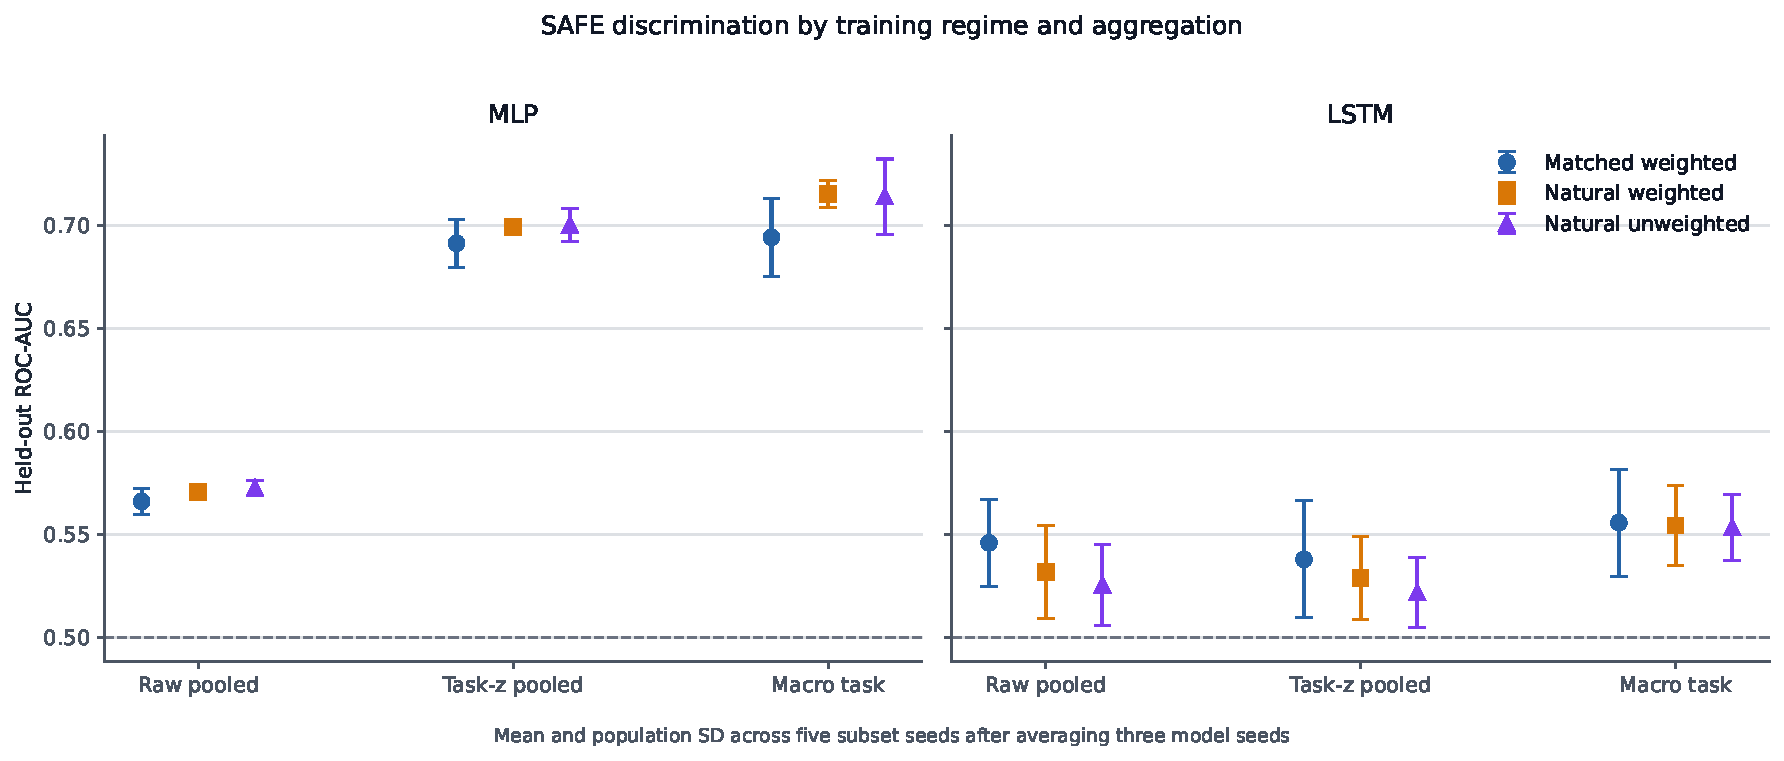
\includegraphics[width=0.93\textwidth]{natural_rate_aggregation.pdf}
\caption{Aggregation view and sampling regime. Natural prevalence and weighting effects are small compared with the difference between raw and task-aware aggregation.}
\end{figure}

For the MLP, natural minus matched was $+0.008\pm0.012$ in task-z ROC and $+0.021\pm0.013$ in macro task ROC. Official weighting minus unweighted natural training was $-0.001\pm0.007$ and $+0.001\pm0.013$. The finite pool is only mildly imbalanced globally, so this does not contradict the paper's weighting choice; it shows that balancing was not the limiting factor here.

\begin{figure}[H]
\centering
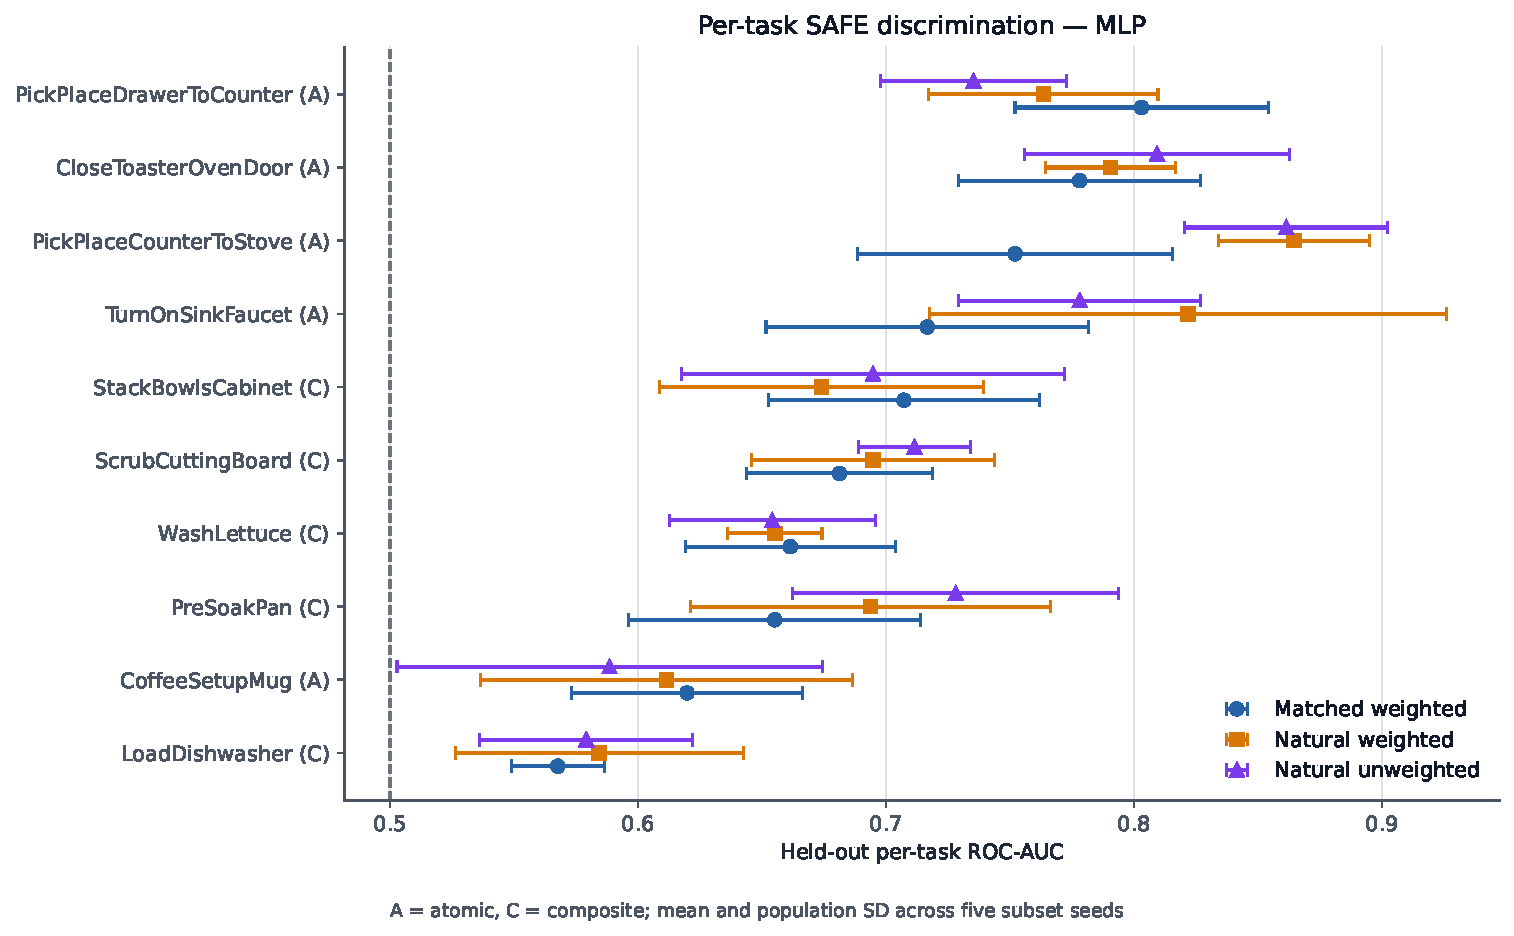
\includegraphics[width=0.92\textwidth]{natural_rate_per_task_mlp.pdf}
\caption{Per-task MLP ROC under the three sampling/weighting regimes. Effects differ by task but do not yield a consistent global advantage.}
\end{figure}

\section{Semantic Subtask-SAFE}

\subsection{Target and decomposition}
The active-stage target is ``does the active natural-language subtask eventually fail before completion?'' A successful parent contributes its completed subtask segments. A failed parent contributes its successful prefix plus exactly one failed active segment; unattempted future stages are excluded.

Predicate-only stages were not sufficient: natural-language tasks can combine several predicates, and adjacent actions may share a predicate. The final schema uses ordered task instructions, merges repeated-predicate stages, drops reset-satisfied stages, and preserves merge provenance.

\subsection{Dataset and grouped split}
Five composite tasks yielded 150 parents and 426 usable segments across 18 task/subtask identities. Failure support is sparse and skewed.

\begin{table}[H]
\centering
\caption{Subtask-SAFE data and outer split.}
\begin{tabular}{lrrrr}
\toprule
Split & Parents & Segments & Success segments & Failure segments\\
\midrule
Training & 100 & 292 & 236 & 56\\
Held-out test & 50 & 134 & 105 & 29\\
Total & 150 & 426 & 341 & 85\\
\bottomrule
\end{tabular}
\end{table}

\begin{figure}[H]
\centering
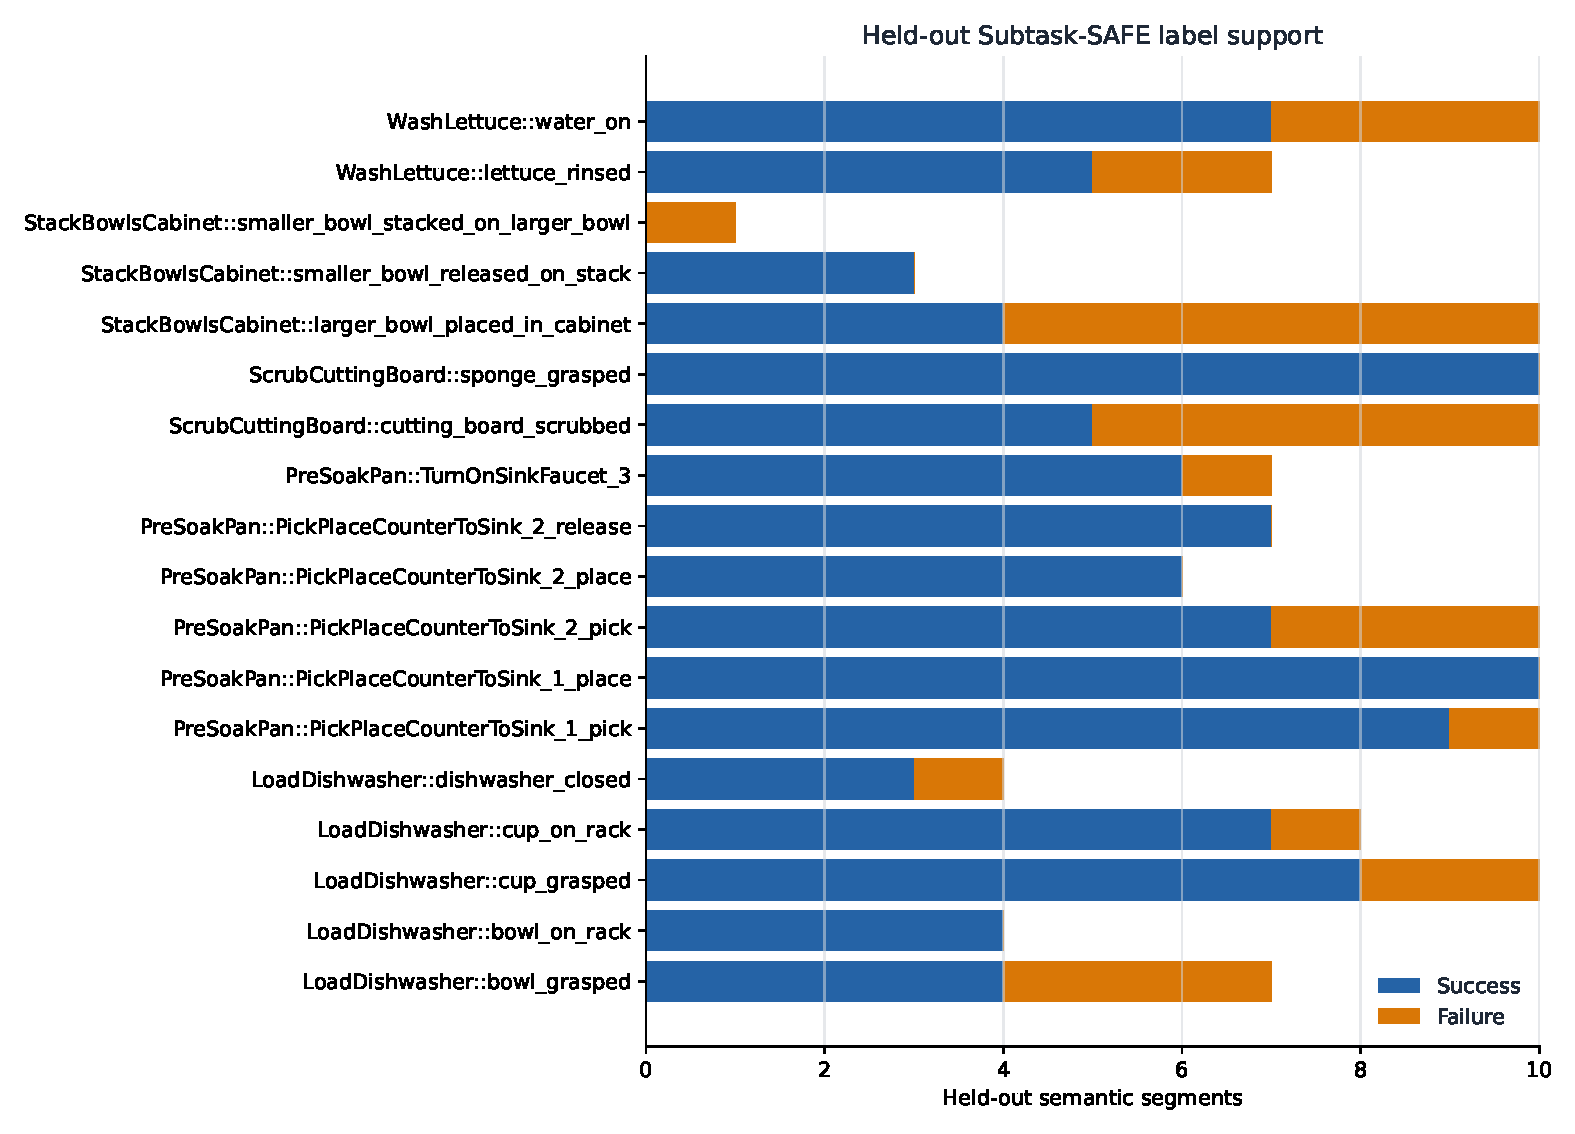
\includegraphics[width=0.96\textwidth]{subtask_per_stage_support.pdf}
\caption{Support by semantic task/subtask identity. Early successful-prefix stages dominate; several stages have little or no failure support.}
\end{figure}

\subsection{Inner CV and retrospective final result}
All 810 inner-CV fits completed. MLP selection was horizon \code{concat-2}, diffusion \code{concat-2}, learning rate $10^{-3}$, regularization $10^{-3}$, with inner ROC $0.749\pm0.037$. LSTM inner ROC was $0.722\pm0.009$.

All six final refits completed with official inverse-frequency class weights $[5.1228,1.2321]$.

\begin{figure}[H]
\centering
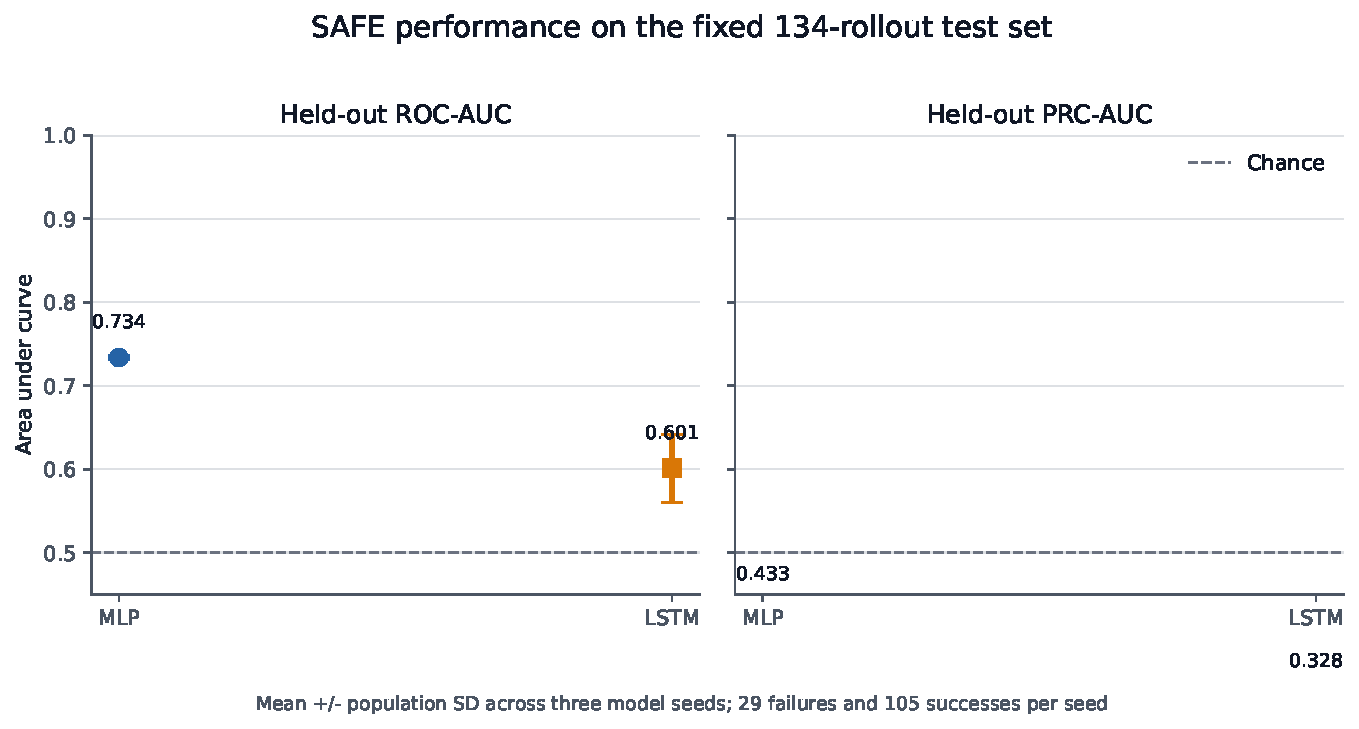
\includegraphics[width=0.76\textwidth]{subtask_test_auc.pdf}
\caption{Retrospective held-out segment discrimination. MLP raw ROC is 0.734, but this uses the full active segment and pools heterogeneous stages.}
\end{figure}

The final retrospective results were MLP ROC $0.734\pm0.002$, PRC $0.433\pm0.012$; LSTM ROC $0.601\pm0.041$, PRC $0.328\pm0.056$. These values motivated, but do not replace, causal evaluation.

\begin{figure}[H]
\centering
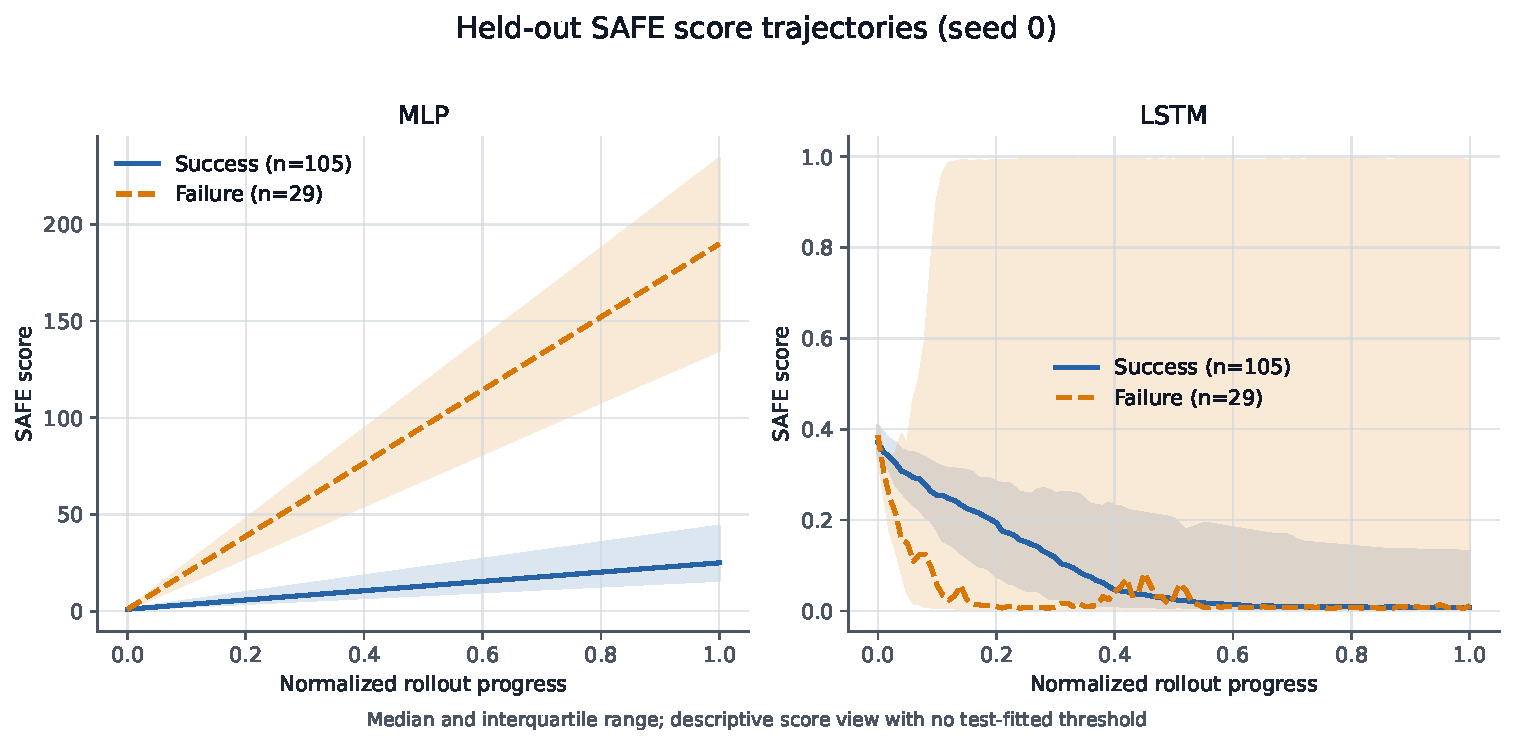
\includegraphics[width=0.98\textwidth]{subtask_score_trajectories.pdf}
\caption{Example retrospective score trajectories. The detector often separates classes only after substantial within-stage evidence has accumulated.}
\end{figure}

\section{Parent-aware causal analysis}

\subsection{Normalization and hierarchical uncertainty}
Raw pooled MLP ROC was 0.734. Training-only task/subtask-z pooling reduced it to $0.561\pm0.025$. A parent-rollout bootstrap gave mean 0.558, 95\% CI [0.428, 0.676]. The elapsed-time baseline achieved mean 0.740, 95\% CI [0.646, 0.827].

\begin{figure}[H]
\centering
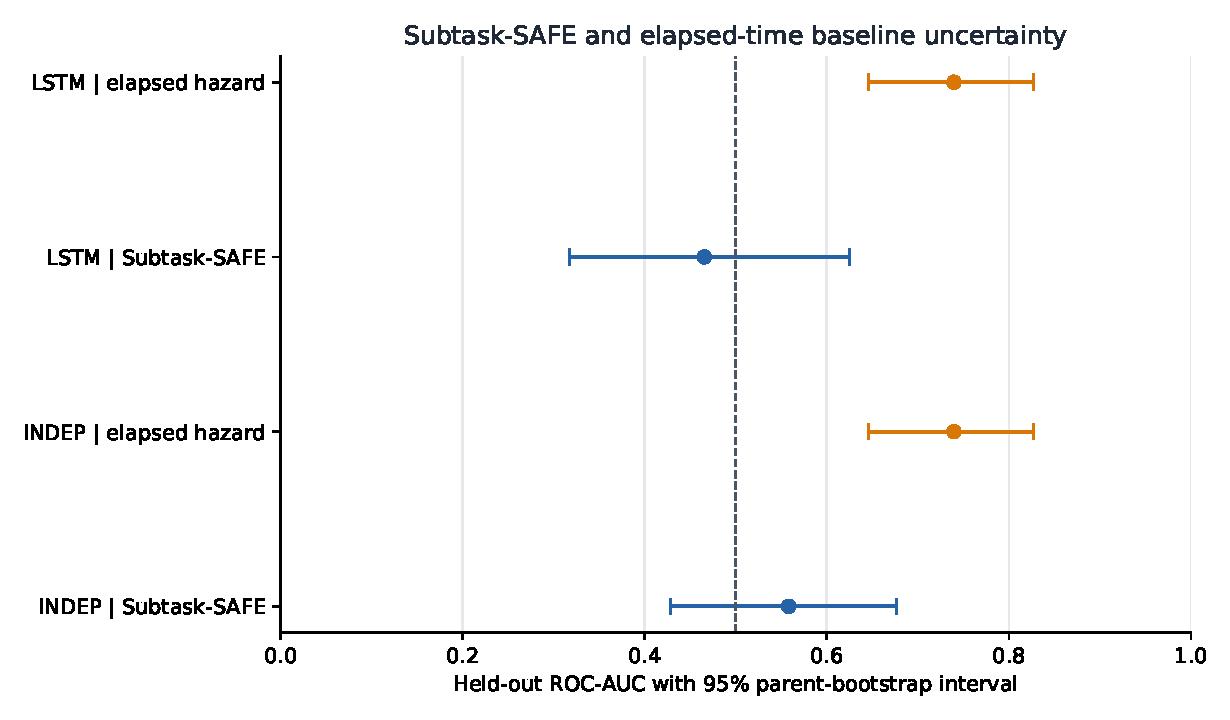
\includegraphics[width=0.88\textwidth]{subtask_parent_bootstrap.pdf}
\caption{Hierarchical parent-rollout bootstrap. SAFE uncertainty overlaps chance, while elapsed time remains consistently stronger.}
\end{figure}

\subsection{Causal prefix test}
Scores were recomputed using only the first $k$ true policy inferences of each active segment. This prevents future within-segment evidence from leaking into an early-warning claim.

\begin{table}[H]
\centering
\caption{Causal-prefix ROC. Counts decrease because shorter segments are ineligible at longer prefixes.}
\begin{tabular}{rrrrr}
\toprule
$k$ & Active segments & MLP SAFE & LSTM SAFE & Elapsed time\\
\midrule
1 & 134 & 0.389 & 0.340 & \textbf{0.742}\\
2 & 127 & 0.347 & 0.363 & \textbf{0.723}\\
4 & 120 & 0.330 & 0.380 & \textbf{0.704}\\
8 & 102 & 0.322 & 0.397 & \textbf{0.685}\\
16 & 68 & 0.374 & 0.463 & \textbf{0.668}\\
32 & 25 & 0.426 & 0.478 & \textbf{0.614}\\
\bottomrule
\end{tabular}
\end{table}

\begin{figure}[H]
\centering
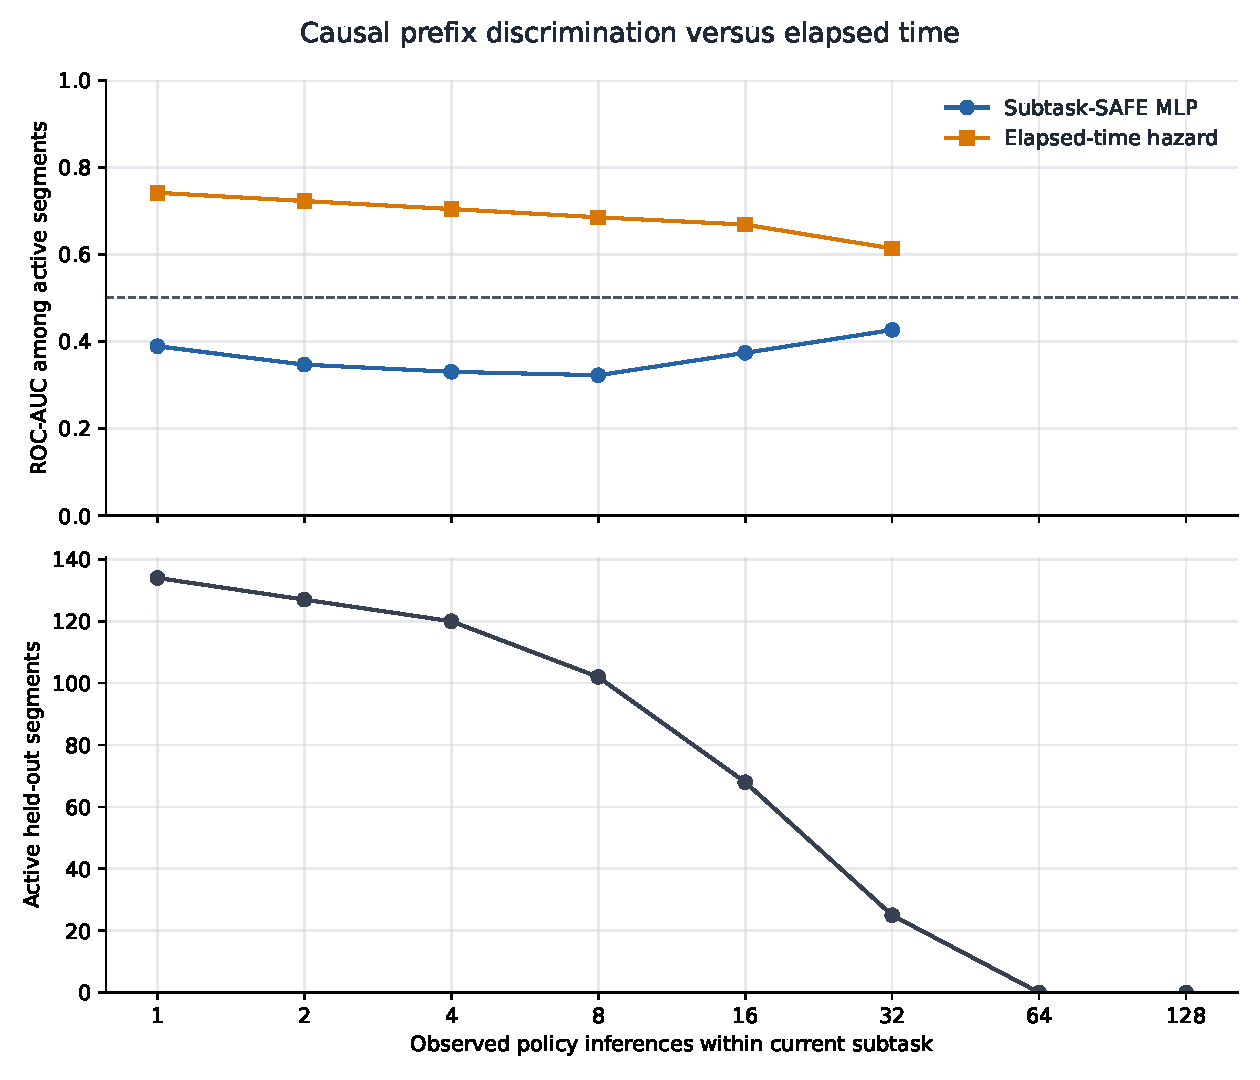
\includegraphics[width=0.94\textwidth]{subtask_causal_prefix_roc.pdf}
\caption{Causal-prefix analysis. Current SAFE scores are below chance at early prefixes; elapsed time is the dominant baseline at every supported prefix.}
\end{figure}

\subsection{Parent-disjoint conformal operation}
Calibration used 15 parents and evaluation used 35 disjoint parents. Reference and nonconformity calibration parents were disjoint. At $\alpha=0.15$, SAFE achieved TPR 0.121, FPR 0.119, balanced accuracy 0.501. Elapsed time achieved TPR 0.500, FPR 0.149, balanced accuracy 0.675.

\begin{figure}[H]
\centering
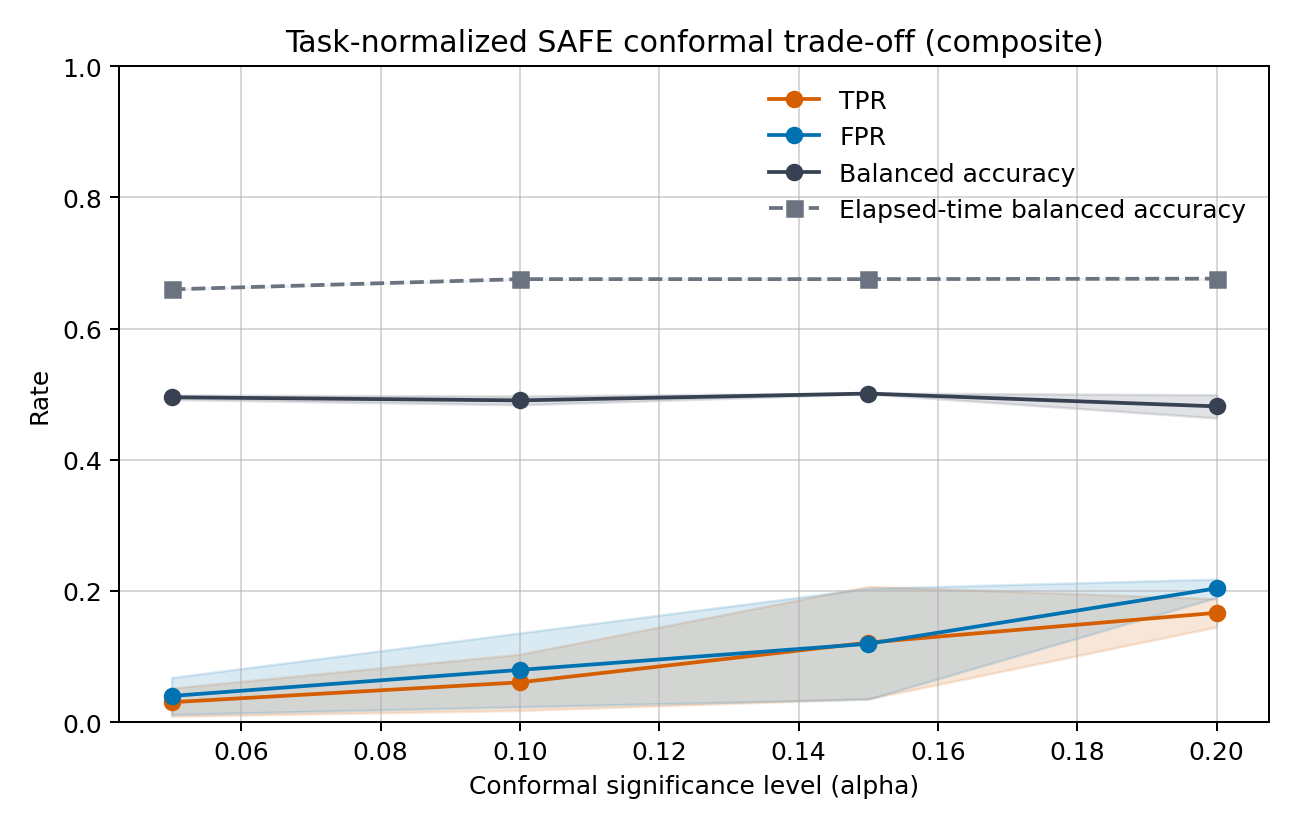
\includegraphics[width=0.92\textwidth]{subtask_conformal_tradeoff.png}
\caption{Parent-disjoint conformal trade-off. SAFE remains near chance across $\alpha$; elapsed time yields materially better balanced accuracy.}
\end{figure}

The reported SAFE lead of 1,661 environment steps at $\alpha=0.15$ applies only to the 12.1\% of failures detected. Lead time without detection coverage would be misleading.

\section{Subtask-SAFE V2: causal objective and frozen evaluation}

\subsection{Continuation gates and four-stage pilot}
The first causal analysis showed that full-segment discrimination was not a sufficient continuation criterion. V2 therefore introduced four explicit gates: causal-prefix performance, comparison with stage-conditioned elapsed time, parent-bootstrap uncertainty, and an operating point with useful TPR, controlled FPR, and positive lead. The data plan initially selected four stages with both scientific value and some failure support:
\begin{itemize}
\item \code{LoadDishwasher::cup\_on\_rack};
\item \code{PreSoakPan::TurnOnSinkFaucet\_3};
\item \code{ScrubCuttingBoard::cutting\_board\_scrubbed};
\item \code{WashLettuce::water\_on}.
\end{itemize}
Their combined segment deficit was 127. Stage-only conditioning gave mean fold ROC approximately 0.599, while stage plus elapsed progress gave approximately 0.588. A broader policy-only/random-prefix ablation selected horizon \code{concat-2}, diffusion selector 1.0, learning rate $3\times10^{-4}$, and regularization 0.01, with inner-validation ROC $0.645\pm0.040$.

The first gated refit did not justify more undirected collection. Its causal-prefix ROC was 0.575 versus 0.673 for elapsed time; TPR was 0.854 only because FPR rose to 0.851. The parent-bootstrap interval for SAFE minus elapsed ROC was $[-0.240,0.037]$. This result motivated a change from the terminal segment label to a within-horizon event target.

\subsection{Within-horizon labels and representation screen}
For a prefix ending at inference $t$, the V2 label asks whether the active stage fails within the next $H$ policy inferences. A feasibility scan showed that $H=128$ with evaluation prefix 32 was the most robust candidate: all three inner folds retained both classes. By contrast, $H=96$ at prefix 48 produced fold ROCs 0.717, 0.250, and 0.400, indicating unstable support.

Fifteen representation/objective treatments were compared on the feasible pilot. Table~\ref{tab:v2-screen} lists the highest-ranking choices. The official SAFE loss on raw features ranked first; temporal summaries were competitive but not uniformly better.

\begin{table}[H]
\centering
\caption{Top V2 representation/loss treatments in the small within-horizon screen. These are inner-validation results, not frozen-test estimates.}
\begin{tabular}{lcc}
\toprule
Representation and loss & Mean ROC & SD\\
\midrule
Raw, official SAFE & \textbf{0.914} & 0.053\\
Raw + delta + mean + slope, official SAFE & 0.867 & 0.066\\
Raw + delta + mean + slope, BCE & 0.838 & 0.046\\
Raw + delta + mean + slope, focal & 0.822 & 0.053\\
Raw + delta, official SAFE & 0.798 & 0.087\\
\bottomrule
\end{tabular}
\label{tab:v2-screen}
\end{table}

The corresponding small final pilot appeared promising: raw features reached ROC 0.819 and temporal summaries 0.956 at prefix 32. However, stage support was only 1/1, 4/0, 3/5, and 7/0 success/failure examples. Each seed also had only five calibration successes, giving nominal conformal resolution $1/(5+1)=0.167$. At target FPRs up to 0.30 the temporal detector produced zero TPR; relaxing the target to 0.40 yielded realized FPR 0.111 and TPR 0.833. The high ROC was therefore treated as a collection pilot, not as a result.

\subsection{Target-aware collection and immutable allocation}
Targeted collection added 400 new-seed parent rollouts. The initial 80-parent batch exposed that the chosen intermediate stages did not consistently accumulate failures. The viable target set was consequently fixed to:
\begin{itemize}
\item \code{LoadDishwasher::dishwasher\_closed};
\item \code{PreSoakPan::TurnOnSinkFaucet\_3};
\item \code{ScrubCuttingBoard::cutting\_board\_scrubbed};
\item \code{WashLettuce::lettuce\_rinsed}.
\end{itemize}
The long collection contributed 120 LoadDishwasher, 120 PreSoakPan, 20 ScrubCuttingBoard, and 30 WashLettuce parents; an additional 30 WashLettuce parents closed the final deficit. Every source dataset passed the rollout, feature, video, and semantic-segment validators.

Before scoring, an immutable target-aware allocation selected five successful calibration parents and 10 successful plus 10 failed evaluation parents per stage. Thus calibration contains 20 parents and evaluation contains 80, with no identity overlap. The remaining 180 eligible new-seed parents were later added to training, while the frozen 100-parent allocation remained byte-for-byte unchanged. The final training manifest contains 280 parents, of which 244 reach a selected target stage; the original old test parents were excluded.

\subsection{Frozen-holdout result}
On the expanded training set, raw inner CV selected horizon \code{concat-2}, diffusion 1.0, learning rate $3\times10^{-5}$, and regularization 0.001, with ROC $0.712\pm0.078$. Temporal summaries selected horizon 1.0, diffusion 1.0, learning rate $10^{-4}$, and regularization 0.001, with ROC $0.703\pm0.029$.

Evaluation at the predeclared causal prefix 32 reversed the optimistic pilot. Raw features achieved ROC $0.512\pm0.003$; raw plus delta, mean, and slope achieved $0.566\pm0.004$. Figure~\ref{fig:v2-frozen-prefix} shows the stage-level heterogeneity.

\begin{figure}[H]
\centering
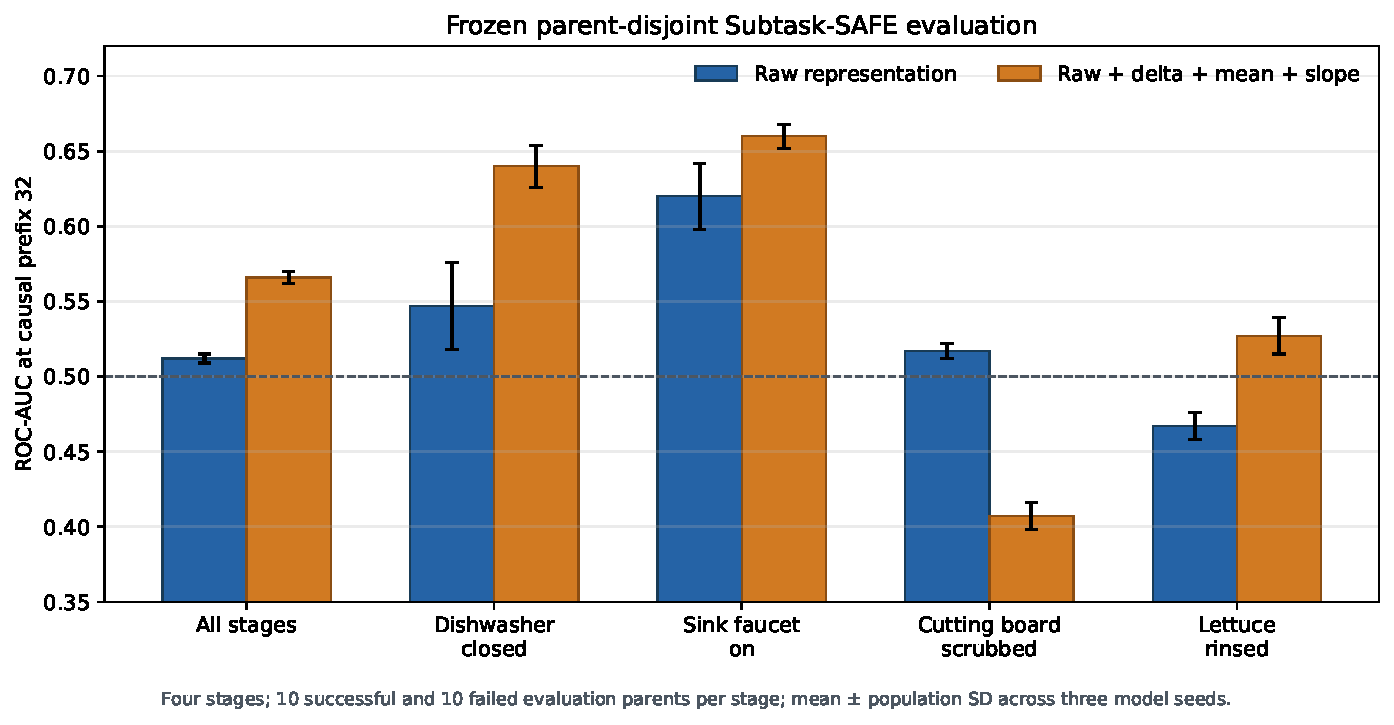
\includegraphics[width=0.98\textwidth]{subtask_v2_frozen_prefix32.pdf}
\caption{Final V2 result on the frozen 80-parent evaluation allocation at causal prefix 32. Each stage contains 10 successful and 10 failed parents. Temporal summaries help on dishwasher closure and faucet activation, hurt cutting-board scrubbing, and remain inconclusive overall.}
\label{fig:v2-frozen-prefix}
\end{figure}

\begin{table}[H]
\centering
\caption{Frozen prefix-32 ROC-AUC, mean $\pm$ population SD across three model seeds.}
\resizebox{\textwidth}{!}{%
\begin{tabular}{lcc}
\toprule
Evaluation group & Raw & Raw + delta + mean + slope\\
\midrule
All four stages & $0.512\pm0.003$ & $\mathbf{0.566\pm0.004}$\\
Dishwasher closed & $0.547\pm0.029$ & $\mathbf{0.640\pm0.014}$\\
Sink faucet on & $0.620\pm0.022$ & $\mathbf{0.660\pm0.008}$\\
Cutting board scrubbed & $\mathbf{0.517\pm0.005}$ & $0.407\pm0.009$\\
Lettuce rinsed & $0.467\pm0.009$ & $\mathbf{0.527\pm0.012}$\\
\bottomrule
\end{tabular}}
\label{tab:v2-frozen}
\end{table}

All-prefix segment ROC was 0.733 for raw features and 0.738 for temporal summaries, but those values pool 675 prefix examples from multiple times and are not the early-warning endpoint. At prefix 32, raw operation gave TPR 0.217, FPR 0.083, and normalized lead 0.755; temporal operation gave TPR 0.133, FPR 0.142, and lead 0.779. Parent-bootstrap confidence intervals for SAFE ROC included chance, and SAFE-minus-duration intervals included zero. Both treatments therefore failed the continuation gates.

This is the most important negative result in the report: additional target-aware data greatly improved class support but did not produce task-robust early discrimination. The large pilot-to-frozen gap shows why target identities and allocation must be frozen before representation selection.

\section{Xiaomi-Robotics-1 original SAFE}

\subsection{Scope and initial ten-task study}
Every Xiaomi result uses only the original binary terminal task label. No
Subtask-SAFE, progress predicate, recovery annotation, or failure-onset label
is present. The initial set contained:
\begin{itemize}
\item five atomic tasks: CoffeeSetupMug, TurnOnMicrowave, TurnOffStove,
CloseBlenderLid, and SlideDishwasherRack;
\item five composites: DeliverStraw, ArrangeTea, WashFruitColander,
GarnishPancake, and WaffleReheat.
\end{itemize}

The first 500 natural rollouts contained 266 successes and 234 failures.
Additional attempts were retained until each task had at least 25 of both
outcomes, producing a 692-rollout pool with 419 successes and 273 failures.
A deterministic seed-0 selection yielded an official-loader-compatible
500-rollout export with exactly 25 successes and 25 failures per task and
40,160 policy records.

\begin{table}[H]
\centering
\caption{Initial Xiaomi 10-task selection and final held-out results. Hyperparameters were selected without using the 160-rollout outer test.}
\begin{tabular}{lccccc}
\toprule
Model & Selected $(h,d,\mathrm{lr},\lambda)$ & Inner ROC & Test ROC & Test AP & Duration ROC\\
\midrule
MLP & $(1,1,10^{-4},10^{-3})$ & $0.534\pm0.008$ & $0.517\pm0.001$ & --- & 0.743\\
LSTM & $(\mathrm{c2},1,10^{-3},10^{-2})$ & $0.595\pm0.029$ & $0.550\pm0.024$ & --- & 0.743\\
\bottomrule
\end{tabular}
\end{table}

At fixed conformal $\alpha=0.15$, normalized MLP and LSTM balanced accuracy was
$0.499\pm0.014$ and $0.522\pm0.038$, respectively. Matched-success-length and
fixed-25\%-landmark controls removed most duration discrimination but did not
produce a strong detector: their best outer ROC values were 0.546 for MLP and
0.530 for LSTM. A causal-prefix experiment reached MLP task-macro ROC 0.610 at
10\% and 0.608 at 25\%, but a staged cascade beat time-only on only two of 240
seed-level failed predictions. This motivated broader collection.

\subsection{Official mid-success task collection}
The broad task set was frozen from Xiaomi's released 2,500-rollout
RoboCasa365 summary. The inclusive selection rule was 5 through 45 successes
out of 50. It selected 39 tasks; tasks at 0/50 or 50/50 were excluded. Two
resumable GPU shards collected exactly 50 new natural rollouts per task with
base seed 100007. All successes, failures, quota overshoot, and historical
errors were preserved.

\begin{longtable}{p{0.32\textwidth}p{0.14\textwidth}rrr}
\caption{Official Xiaomi success count and the new 50-rollout collection.}\\
\toprule
Task & Type & Official & Fresh success & Fresh failure\\
\midrule
\endfirsthead
\toprule
Task & Type & Official & Fresh success & Fresh failure\\
\midrule
\endhead
CategorizeCondiments & composite & 5 & 7 & 43\\
PrepareCoffee & composite & 8 & 9 & 41\\
PortionHotDogs & composite & 10 & 8 & 42\\
SearingMeat & composite & 13 & 15 & 35\\
PackIdenticalLunches & composite & 14 & 14 & 36\\
WeighIngredients & composite & 14 & 15 & 35\\
BreadSelection & composite & 15 & 17 & 33\\
CuttingToolSelection & composite & 17 & 22 & 28\\
RecycleBottlesByType & composite & 17 & 9 & 41\\
CloseBlenderLid & atomic & 18 & 17 & 33\\
GetToastedBread & composite & 18 & 20 & 30\\
MakeIceLemonade & composite & 19 & 19 & 31\\
StirVegetables & composite & 19 & 24 & 26\\
WaffleReheat & composite & 21 & 29 & 21\\
ArrangeTea & composite & 23 & 27 & 23\\
DeliverStraw & composite & 23 & 18 & 32\\
CoffeeSetupMug & atomic & 25 & 20 & 30\\
WashFruitColander & composite & 27 & 31 & 19\\
TurnOnMicrowave & atomic & 28 & 33 & 17\\
GarnishPancake & composite & 29 & 31 & 19\\
ArrangeBreadBasket & composite & 30 & 25 & 25\\
RinseSinkBasin & composite & 30 & 35 & 15\\
TurnOffStove & atomic & 30 & 30 & 20\\
SteamInMicrowave & composite & 32 & 35 & 15\\
LoadDishwasher & composite & 36 & 36 & 14\\
SetUpCuttingStation & composite & 36 & 32 & 18\\
StackBowlsCabinet & composite & 36 & 40 & 10\\
KettleBoiling & composite & 37 & 29 & 21\\
PreSoakPan & composite & 38 & 38 & 12\\
ScrubCuttingBoard & composite & 40 & 35 & 15\\
SlideDishwasherRack & atomic & 40 & 42 & 8\\
StoreLeftoversInBowl & composite & 42 & 43 & 7\\
TurnOnSinkFaucet & atomic & 42 & 38 & 12\\
WashLettuce & composite & 42 & 36 & 14\\
PickPlaceCounterToCabinet & atomic & 43 & 44 & 6\\
PickPlaceSinkToCounter & atomic & 44 & 49 & 1\\
CloseToasterOvenDoor & atomic & 45 & 44 & 6\\
OpenCabinet & atomic & 45 & 46 & 4\\
PickPlaceCounterToStove & atomic & 45 & 44 & 6\\
\midrule
\textbf{Total} & 39 tasks & --- & \textbf{1,106} & \textbf{844}\\
\bottomrule
\end{longtable}

Deep validation found 1,950 unique rollout IDs and task/seed/reset identities,
no missing required artifacts, and no loader incompatibility. Twelve historical
error records document recovered attempts. The two shards occupied about
36 GiB.

\subsection{Pooling, split, and detector selection}
The 1,950 new rollouts were merged with the earlier 692, giving an immutable
2,642-rollout pool. Deterministic within-task/outcome selection retained
exactly 50 per task: 1,105 successes and 845 failures. The
\code{PickPlaceSinkToCounter} group had only one failure and was excluded from
model development, leaving 38 tasks.

\begin{table}[H]
\centering
\caption{Frozen broad Xiaomi split and hyperparameter search.}
\begin{tabular}{lr}
\toprule
Property & Value\\
\midrule
Outer training & 1,824 (1,018 success; 806 failure)\\
Untouched outer test & 76 (38 success; 38 failure)\\
Held-out support & 1 success and 1 failure per task\\
Grid & $3h\times3d\times5$ learning rates $\times3$ regularizers\\
Inner folds/model seeds & 3 / 3\\
Completed fits & 810/810; zero failures\\
\bottomrule
\end{tabular}
\end{table}

The MLP selected $(h=1,d=1,\mathrm{lr}=10^{-4},\lambda=10^{-3})$ with inner
ROC $0.654\pm0.025$. The LSTM selected
$(h=\mathrm{concat\mbox{-}2},d=\mathrm{concat\mbox{-}2},
\mathrm{lr}=3\times10^{-4},\lambda=0.1)$ with inner ROC
$0.742\pm0.012$. All six final refits completed on identical identities.

\begin{table}[H]
\centering
\caption{Broad Xiaomi final refits and training-only task normalization.}
\begin{tabular}{lccccc}
\toprule
Model & Raw ROC & Task-z ROC & Raw AP & Task-z AP & Macro task ROC\\
\midrule
MLP & $0.532\pm0.016$ & $\mathbf{0.692\pm0.013}$ & 0.528 & \textbf{0.733} & \textbf{0.689}\\
LSTM & $0.628\pm0.008$ & $0.646\pm0.017$ & 0.640 & 0.663 & 0.640\\
\bottomrule
\end{tabular}
\end{table}

Completed-duration ROC was 0.804. Normalization reversed the raw architecture
ordering: the MLP has the best within-task ranking, whereas the LSTM benefits
more from between-task score offsets.

\subsection{Atomic/composite and causal online replay}
The 38-task set contains ten atomic and 28 composite tasks. Because each task
has only one held-out example per class, the task-type estimates are imprecise.

\begin{table}[H]
\centering
\caption{Atomic versus composite outer-test results.}
\resizebox{\textwidth}{!}{%
\begin{tabular}{lllccccc}
\toprule
Model & Type & Tasks & Raw ROC & Task-z ROC & Task-z AP & Macro ROC & Time ROC\\
\midrule
MLP & Atomic & 10 & $0.573\pm0.045$ & $0.730\pm0.054$ & $0.792\pm0.053$ & 0.600 & 1.000\\
MLP & Composite & 28 & $0.539\pm0.018$ & $0.680\pm0.025$ & $0.729\pm0.015$ & $0.720\pm0.017$ & 0.912\\
LSTM & Atomic & 10 & $0.627\pm0.098$ & $0.630\pm0.123$ & $0.727\pm0.098$ & $0.633\pm0.125$ & 1.000\\
LSTM & Composite & 28 & $0.660\pm0.027$ & $0.651\pm0.021$ & $0.647\pm0.019$ & $0.643\pm0.051$ & 0.912\\
\bottomrule
\end{tabular}}
\end{table}

The MLP macro atomic-minus-composite difference was -0.120, with task-bootstrap
95\% interval $[-0.416,0.166]$; the LSTM difference was -0.010 with interval
$[-0.264,0.245]$. No reliable task-type difference is established.

Causal replay used only the current prefix, task identity, training-derived
horizon, and active status. It split the 1,824 training rollouts into 1,748
meta-fit and 76 threshold-validation rollouts; the opened 76-rollout outer test
was unchanged.

\begin{table}[H]
\centering
\caption{Causal online event replay. Detection is fraction of task horizon; adjusted assigns missed failures 1.0.}
\resizebox{\textwidth}{!}{%
\begin{tabular}{lllcccccc}
\toprule
Model & Detector & Event ROC & TPR & FPR & Balanced accuracy & Detection & Adjusted\\
\midrule
MLP & Time only & 0.965 & 0.842 & 0.053 & 0.895 & 0.786 & 0.820\\
MLP & SAFE only & $0.951\pm0.011$ & $0.983\pm0.025$ & 0.132 & $0.925\pm0.012$ & $0.662\pm0.021$ & $0.668\pm0.028$\\
MLP & SAFE+time+task & $0.968\pm0.007$ & $0.965\pm0.025$ & 0.053 & $0.956\pm0.012$ & $0.842\pm0.013$ & $0.848\pm0.008$\\
LSTM & SAFE only & $0.814\pm0.032$ & $0.895\pm0.057$ & $0.377\pm0.054$ & $0.759\pm0.033$ & $0.346\pm0.032$ & $0.415\pm0.049$\\
LSTM & SAFE+time+task & $0.863\pm0.019$ & $0.781\pm0.090$ & $0.272\pm0.045$ & $0.754\pm0.022$ & $0.435\pm0.040$ & $0.556\pm0.074$\\
\bottomrule
\end{tabular}}
\end{table}

At fixed causal landmarks, MLP SAFE task-macro ROC was 0.671 at 10\% and
0.626 at 25\%; LSTM values were 0.667 and 0.616. Task-conditioned time-only is
exactly 0.5 within task at a fixed landmark. This is evidence of early internal
signal, but not yet of a better operating policy: MLP SAFE obtains earlier
detection by accepting five false alarms among 38 successes, versus two for
time-only.

\subsection{Frozen prospective matched-FPR experiment}
The confirmatory next step is a two-phase shadow protocol. It preserves all
three selected MLP seeds, fits per-seed normalization from the original 1,824
training rollouts, takes each seed's running maximum, and averages the three
normalized trajectories. A new calibration batch targets three successes and
three failures per task (228 primary outcome-quota rollouts, plus retained
overshoot). It
selects global thresholds under one empirical event-level
$\mathrm{FPR}\leq0.05$ constraint. The staged detector permits SAFE from rollout
start through 25\%, suppresses alarms from 25--50\%, and enables the frozen
task-conditioned time fallback from 50\% onward. Its two thresholds are searched
jointly under the same rollout-level FPR cap.

After the runtime bundle is frozen, a disjoint shadow test targets ten
successes and ten failures per task (760 primary outcome-quota rollouts, plus
retained overshoot). Frozen thresholds are replayed causally at every recorded
inference, but never stop, retry, recover, or change the Xiaomi policy. Primary
endpoints are Wilson-interval TPR/FPR,
miss-adjusted detection fraction, recall by 10/25/50\%, paired
earlier/same/later/missed counts, task-macro landmark ROC, task/rollout
bootstrap intervals, FPR drift, and atomic/composite strata.

The staged detector passes only if FPR remains compatible with 5\%, TPR is no
more than 0.05 below time-only, adjusted detection is at least 0.10 earlier,
at least 25\% of failures are detected by 25\%, and the paired bootstrap favors
earlier detection without material excess false alarms. Recovery is a separate
randomized intervention experiment and is not estimated from shadow data.

\section{Interpretation across all experiments}

\subsection{What the evidence supports}
\begin{enumerate}
\item The feature-capture and official-export engineering is valid for both $\pi_0$ and RLDX.
\item RLDX MLP features contain useful within-task retrospective failure information.
\item Atomic tasks are materially easier than composite tasks.
\item Task and stage score offsets are large; task-aware normalization is reasonable when fitted without test leakage and when task identity is available.
\item Semantic decomposition is necessary for valid subtask labels and grouped evaluation.
\item Parent-aware causal-prefix testing is necessary before claiming early warning.
\item A frozen, stage-balanced evaluation allocation prevents promising but support-limited pilot results from becoming final claims.
\item Xiaomi's normalized MLP contains early within-task causal signal across a much broader task set, making it the current best candidate for a matched-FPR shadow test.
\end{enumerate}

\subsection{What the evidence rejects}
\begin{enumerate}
\item More complex temporal modeling alone: the LSTM was not competitive.
\item Mixed horizons alone as the cause: split atomic/composite models did not beat the mixed MLP.
\item Balanced sampling alone as the cause: natural prevalence and paper-style weighting had negligible paired effects.
\item Semantic decomposition alone as the solution: Subtask-SAFE raw ROC did not translate into early causal discrimination.
\item Within-horizon relabeling, stage conditioning, and temporal summaries as sufficient fixes: all improved selected pilots, but failed to transfer to the immutable four-stage test.
\item More of the same target-aware data as a guaranteed remedy: expanding to 280 training parents did not make prefix-32 ROC statistically distinguishable from chance.
\item Raw pooled Xiaomi scores as the deployment variable: training-only task normalization is necessary for the MLP, and elapsed time remains a stronger raw retrospective predictor.
\end{enumerate}

\subsection{Why normalization is reasonable, but insufficient}
Training-only task or task/subtask normalization is scientifically reasonable because different tasks have different score scales and the deployed controller knows its commanded task. It is analogous to task-conditional calibration, not test-set tuning. However, normalization can only remove offsets; it cannot create within-stage ordering. The Subtask-SAFE drop from raw ROC 0.734 to parent-aware 0.558 exposes that limitation. Xiaomi is the complementary case: MLP task-z ROC rises from 0.532 to 0.692, indicating useful within-task ordering hidden by task offsets. Every policy family still requires its own training-derived calibration; thresholds and normalization are not transferable.

\section{Recommended next experiments}

\begin{enumerate}
\item \textbf{Run the Xiaomi prospective matched-FPR shadow test first.} Use the already selected three-seed MLP ensemble, a fresh 3/3-per-task calibration batch, a disjoint 10/10-per-task test, a jointly constrained 5\% FPR cascade, and no policy intervention.
\item \textbf{Freeze before test collection.} Persist checkpoint and config checksums, training-only normalization, task horizons, time-risk curves, thresholds, stage windows, task list, and calibration identities. Never retune these values after test outcomes are visible.
\item \textbf{Retain every attempt.} Outcome quotas define the primary balanced endpoint, while the complete overshoot stream supplies an all-retained sensitivity analysis and documents collection cost and errors. Because stopping depends on both class quotas, this stream is not an unbiased deployment-prevalence sample.
\item \textbf{Keep paired timeliness primary.} Compare staged SAFE and time-only on identical failed rollouts with misses assigned fraction 1.0; report recall by 10/25/50\%, Wilson intervals, and task/rollout bootstrap differences.
\item \textbf{Gate recovery on the frozen success criteria.} Only a prospective pass permits a separately powered randomized shadow-versus-recovery intervention study.
\item \textbf{Continue RLDX diagnosis separately.} Stage-specific heads, survival objectives, earlier feature layers, and complementary proprioceptive/contact signals remain appropriate RLDX follow-ups, but they must not be mixed with Xiaomi original-SAFE evidence.
\end{enumerate}

\section{Limitations}
\begin{itemize}
\item $\pi_0$ and RLDX use different policies, feature shapes, tasks, and data volumes; absolute values are not direct architecture comparisons.
\item Only three detector seeds were used; $\pi_0$ held-out sets were particularly small.
\item Natural-rate subsets reflect the collected pool, not an unconstrained deployment distribution.
\item Failure support is sparse for many semantic stages; segment classes are strongly imbalanced.
\item Segments within one parent are dependent; only the parent-aware analyses model this hierarchy explicitly.
\item The original causal-prefix study falls to 25 segments at 32 inferences and zero at 64; V2 fixes prefix-32 balance for four stages but does not test unseen task identities.
\item The frozen 100-parent allocation was inspected in an earlier target-aware experiment before the augmented refit. It is a locked paired follow-up set, not a pristine new confirmatory test.
\item Only four composite stages have balanced V2 evaluation support; per-stage confidence remains limited at 10 successes and 10 failures.
\item RoboCasa predicate boundaries are privileged simulator information; a real robot requires a separate online subtask-progress estimator.
\item Conformal validity depends on exchangeability and can fail under task, policy, layout, or seed drift.
\item The broad Xiaomi outer test has only one success and one failure per task; task-level and atomic/composite uncertainty is therefore wide.
\item Xiaomi causal replay is post-hoc because the 76 outer-test trajectories were already opened by raw and normalized analyses.
\item The prospective Xiaomi calibration and test described here were not yet run at report time; their sample counts are minimum targets, not completed evidence.
\end{itemize}

\appendix
\section{Experiment roots}
\small
\begin{longtable}{p{0.26\textwidth}p{0.66\textwidth}}
\toprule
Experiment & Cluster path\\
\midrule
$\pi_0$ official grid & \path{/gs/bs/tga-shinoda/felid/robocasa_checkpoints/safe/safe_pi0_official_grid_2gpu_20260716_153526}\\
$\pi_0$ leakage-free CV & \path{/gs/bs/tga-shinoda/felid/robocasa_checkpoints/safe/safe_all5_seen_innercv_20260717_012538}\\
RLDX 10-task CV & \path{/gs/bs/tga-shinoda/felid/robocasa_checkpoints/safe/safe_rldx1_seen10_official_cv_2gpu_20260727_135354}\\
RLDX 10-task final & \path{/gs/bs/tga-shinoda/felid/robocasa_checkpoints/safe/safe_rldx1_seen10_final_refit_20260727_155824}\\
RLDX 25/25 CV & \path{/gs/bs/tga-shinoda/felid/robocasa_checkpoints/safe/safe_rldx1_25x25_cv_2gpu_20260729_203916}\\
RLDX 25/25 final & \path{/gs/bs/tga-shinoda/felid/robocasa_checkpoints/safe/safe_rldx1_25x25_final_2gpu_20260730_104400}\\
RLDX calibration & \path{/gs/bs/tga-shinoda/felid/robocasa_checkpoints/safe/safe_rldx1_25x25_final_2gpu_20260730_104400_calibration_20260730_113807}\\
RLDX expanded alpha sweep & \path{/gs/bs/tga-shinoda/felid/robocasa_checkpoints/safe/safe_rldx1_25x25_final_2gpu_20260730_104400_alpha_sweep_005_to_050_20260806_142630}\\
Task-type ablation & \path{/gs/bs/tga-shinoda/felid/robocasa_checkpoints/safe/safe_rldx1_25x25_type_ablation_20260730_115819}\\
Natural-rate study & \path{/gs/bs/tga-shinoda/felid/robocasa_checkpoints/safe/safe_rldx1_natural_rate_screen_20260730_161528}\\
Subtask source data & \path{/gs/bs/tga-shinoda/felid/robocasa_rollouts/safe/rldx1_composite_subtask_seed8_9_10_150_20260803_210535}\\
Subtask official export & \path{/gs/bs/tga-shinoda/felid/robocasa_rollouts/safe/rldx1_subtask_safe_official_20260803_212413}\\
Subtask CV & \path{/gs/bs/tga-shinoda/felid/robocasa_checkpoints/safe/rldx1_subtask_safe_cv_2gpu_20260803_222020}\\
Subtask final/causal & \path{/gs/bs/tga-shinoda/felid/robocasa_checkpoints/safe/rldx1_subtask_safe_final_2gpu_20260804_150002}\\
Subtask V2 pilot & \path{/gs/bs/tga-shinoda/felid/robocasa_checkpoints/safe/rldx1_subtask_v2_final_20260804_185021}\\
Target-aware frozen pool & \path{/gs/bs/tga-shinoda/felid/robocasa_rollouts/safe/rldx1_target_aware_holdout400_20260805_162027}\\
Augmented split manifest & \path{/gs/bs/tga-shinoda/felid/robocasa_rollouts/safe/rldx1_subtask_augmented280_frozen100_20260805_190520}\\
Augmented raw/temporal CV & \path{/gs/bs/tga-shinoda/felid/robocasa_checkpoints/safe/rldx1_augmented280_frozen100_cv_2gpu_20260805_205645}\\
Augmented frozen final & \path{/gs/bs/tga-shinoda/felid/robocasa_checkpoints/safe/rldx1_augmented280_frozen100_final_2gpu_20260806_132421}\\
Xiaomi 10-task balanced export & \path{/gs/bs/tga-shinoda/felid/robocasa_rollouts/safe/xr1_safe_balanced_25x25_seed0_20260807_122434/official_safe_25x25_seed0}\\
Xiaomi 39-task collection & \path{/gs/bs/tga-shinoda/felid/robocasa_rollouts/safe/xr1_safe_official_5to45_50each_20260808_215640}\\
Xiaomi 2,642-rollout pool & \path{/gs/bs/tga-shinoda/felid/robocasa_rollouts/safe/xr1_safe_pooled_39tasks_50each_seed0_20260812_221815/source_pool_all_2642}\\
Xiaomi broad final refits & \path{/gs/bs/tga-shinoda/felid/robocasa_checkpoints/safe/xr1_pooled_39tasks_final_refits_20260814_231508}\\
Xiaomi causal replay & \path{/gs/bs/tga-shinoda/felid/robocasa_checkpoints/safe/xr1_pooled_39tasks_final_refits_20260814_231508/causal_online_replay_20260815_003121}\\
\bottomrule
\end{longtable}
\normalsize

\section{Reproducibility and figure map}
The repository chronology is maintained in
\path{docs/safe_robocasa_experiment_report.md}. Core entry points are:
\begin{itemize}
\item \code{collect\_atomic\_rollouts}, \code{collect\_mixed\_rollouts}, and
\code{export\_official\_safe};
\item \code{run\_seen\_cv\_grid} and \code{train\_seen\_tasks};
\item \path{score_seen_checkpoint_external} and
\path{run_prospective_matched_fpr};
\item the parent-aware Subtask-SAFE analysis and calibration modules.
\end{itemize}

Most figures in this PDF are copied unchanged from the checksum-verified evidence bundle. The 6 August comparison and frozen-prefix figures are deterministic renderings of the report CSVs; their generator is \path{generate_update_figures.py}. \path{chart_map.md} records the source path and interpretation for every visual. Machine-readable supporting CSVs are in \path{tables/}. Videos remain in the evidence bundle; they are not embedded in PDF because their timing and score overlays are better inspected as MP4. The score-video tool now supports a full-rollout view and filenames that identify normalization, ground truth, and detector correctness.

\section{Metric-reading checklist}
\begin{enumerate}
\item Is the metric retrospective full-segment or causal-prefix?
\item Is the score raw pooled, train-only normalized, or macro per task/stage?
\item Are dependent segments grouped by parent rollout?
\item Was the outer test excluded from hyperparameter selection and calibration fitting?
\item Is elapsed time evaluated on the same identities?
\item For conformal results, are TPR, FPR, balanced accuracy, and lead time reported together?
\end{enumerate}

\begin{thebibliography}{9}
\bibitem{gu2026safe}
Gu, J., Kirmani, S., et al.
\newblock SAFE: Multitask failure detection for vision-language-action models.
\newblock \emph{Advances in Neural Information Processing Systems}, 2025.
\newblock \href{https://vla-safe.github.io/}{SAFE project page and paper}.
\end{thebibliography}

\end{document}
